\section{Modeling}

\subsection{Problem Setup}
The goal is to classify cloud presence ($+1$ for cloud, $-1$ for not cloud) using Multi-angle Imaging SpectroRadiometer (MISR) radiance data. Our modeling pipeline adopts a temporal holdout strategy: the training set consists of images \texttt{O012791} and \texttt{O013257}, while the image \texttt{O013490} serves as a temporal holdout test set. 
During training and testing, we only use the labeled pixels, 
This split reflects the real-world challenge of deploying a model on future satellite orbits. The features used include the original MISR radiance angles (DF, CF, BF, AF, AN), expert-engineered features (NDAI\_DF\_AF, SD, CORR), and a suite of 32 latent features derived from our autoencoder (AE) model.

\subsection{Models Compared}
There are three machine learning methods we applied, namely Ensemble Learning (including Random Forest and Boosting), Logistic Regression, and Support Vector Machine. For Ensemble Learning, we evaluate four main configurations to understand the impact of feature engineering and regularization:
\begin{enumerate}
    \item \textbf{Random Forest (Literature):} A baseline RF model using only the following three features: \texttt{SD}, \texttt{CORR}, and new \texttt{NDAI\_DF\_AF}.
    \item \textbf{Histogram Gradient Boosting (Base):} An efficient gradient-boosted decision tree implementation utilizing only the 3 literature features and original features(DF, CF, BF, AF, AN).
    \item \textbf{Random Forest (Full):} A Random Forest ensemble trained on all 40 features (8 base + 32 AE).
    \item \textbf{Histogram Gradient Boosting (Full):} The HGB architecture trained on the full 40-feature set.
\end{enumerate}

For Logistic Regression and SVM, we have two variations each:
\begin{enumerate}
    \item \textbf{LASSO Logistic Regression:} A Logistic Regression model with Lasso selecting existing features using L1 penalty.
    \item \textbf{Stepwise Logistic Regression:} Logistic Regression model with features generated by stepwise selection (with accuracy as the scoring criterium).
    \item \textbf{Tuned SVM:} SVM model trained on 8 selected features with its parameters tuned through Grid Search methodology.
    \item \textbf{SVM (Base):} SVM trained on the three engineered features applied in the paper: \texttt{SD}, \texttt{CORR}, and \texttt{NDAI}.
\end{enumerate}

\subsection{Model Assumptions and Reasonableness}
Both Random Forest and Gradient Boosting are tree-based ensemble methods. These models are nonparametric and do not require strong assumptions about the underlying distribution of the data (such as linearity or normality of residuals). However, they are sensitive to covariate shifts between training and testing data.
The logistic regression model assumes a linear relationship between the logit transformation of response variables and the predictor variables. SVM assumes a set of support vectors serving as margins that form a hyperplane in a kernel space to separate the binary categories. Following an extensive grid search for parameter tuning, the L1 penalty coefficient for the Lasso logistic regression was set at 0.8 and the penalty parameter for the support vector machine was fixed at 1.0. \\


We assessed the temporal stability by calculating the Standardized Mean Difference (SMD) and skewness shifts between the training images and the temporal holdout. Significant distribution shifts were observed in several features:
\begin{itemize}
    \item \textbf{NDAI\_DF\_AF:} $|SMD| = 1.147$; training skew = $2.481$, testing skew = $1.226$.
    \item \textbf{DF (Radiance angle):} $|SMD| = 0.748$; training skew = $-0.676$, testing skew = $-1.762$.
    \item \textbf{CORR:} $|SMD| = 0.537$; training skew = $-0.639$, testing skew = $0.099$.
\end{itemize}
Tree-based models remain reasonable choices due to their ability to model complex, non-linear interactions without requiring specific parametric forms, though they must be monitored for performance degradation in new environments, while both Logistic Regression and SVM are intuitively suitable for this research because the fundamental nature of the task is binary classification. 


\subsection{Fit Assessment}
Model performance was evaluated using the temporal holdout test (Table \ref{tab:model_comparison}). All tree models achieved high ROC AUC values ($>0.99$). Interestingly, the literature-based RF performs remarkably well, suggesting the three core features carry the vast majority of the signal. The models with full features provide a slight edge in Accuracy.

\begin{table}[H]
\centering
\begin{tabular}{lccccc}
\toprule
\textbf{Model} & \textbf{Accuracy} & \textbf{ROC AUC} & \textbf{F1 Score} & \textbf{Precision} & \textbf{Recall} \\ 
\midrule
RF (Literature)       & 0.9559 & 0.9945 & 0.9558 & 0.9170 & 0.9981 \\
HGB (Base)  & 0.9608 & 0.9958 & 0.9605 & 0.9283 & 0.9950 \\
RF (Full)             & 0.9732 & 0.9941 & 0.9725 & 0.9564 & 0.9892 \\
HGB (Full)            & 0.9787 & 0.9976 & 0.9780 & 0.9660 & 0.9903 \\
Lasso (Full)       & 0.4973 & 0.5109 & 0.4957 & 0.5148 & 0.5065 \\
StepWise (Full)       & 0.8200 & 0.8101 & 0.8113 & 0.8274 & 0.8148 \\
SVM (Base)       & 0.9563 & 0.9487 & 0.9523 & 0.9465 & 0.9435 \\
SVM (Full)       & 0.4202 & 0.4148 & 0.3569 & 0.5152 & 0.4878 \\
\bottomrule
\end{tabular}
\caption{Performance metrics on the temporal holdout set (\texttt{O013490}). HGB (Base) is selected as the primary model.}
\label{tab:model_comparison}
\end{table}

\subsection{Selected Model Diagnostics (HGB-Base)}
The ROC curve analysis of out selected model (Figure \ref{fig:roc_curve}) shows that while all models perform well, zooming into the top-left corner reveals that HGB-Base and HGB-Full maintain a slightly more "square" curve than the RF variants, like Stepwise Logistic Regression (Figure \ref{fig:bad_roc}).

\begin{figure}[H]
    \centering
    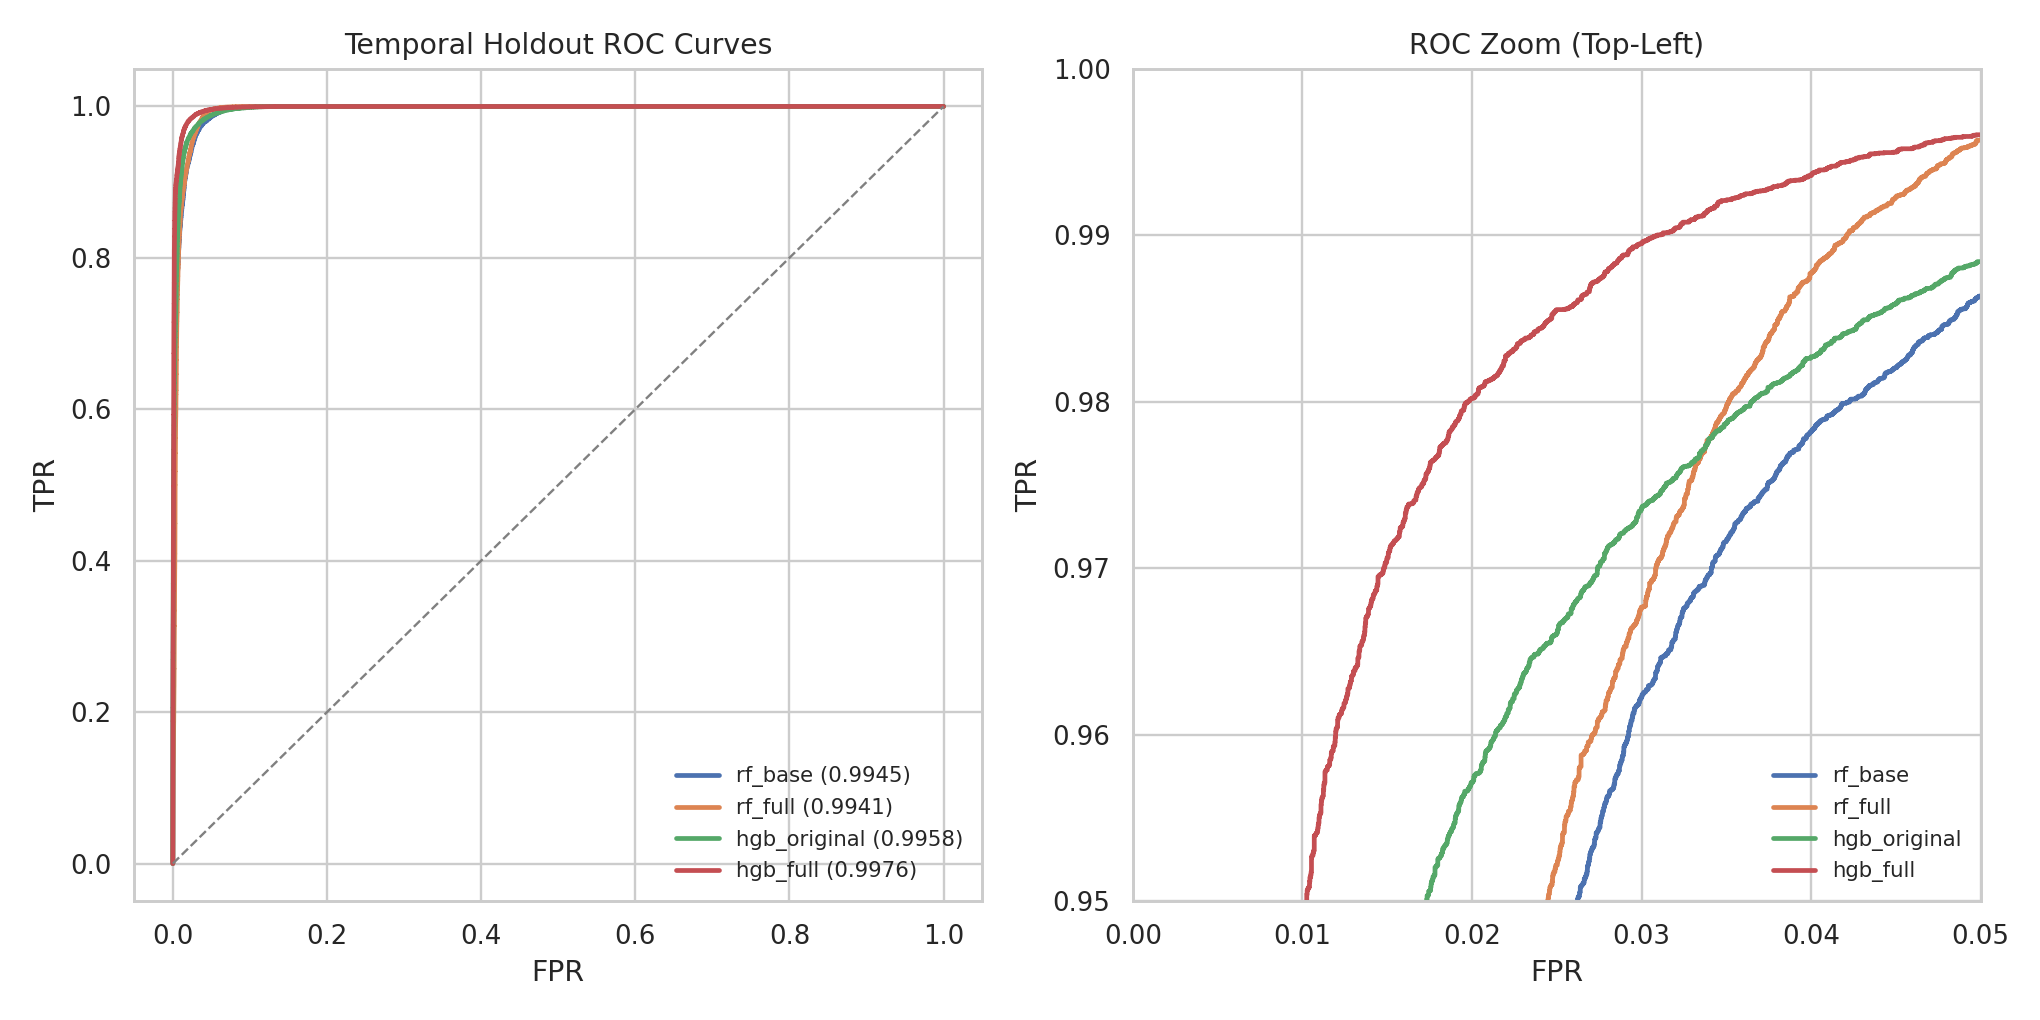
\includegraphics[width=0.9\textwidth]{figures/model/fig_model_roc_temporal_holdout.png}
    \caption{Temporal Holdout ROC Curves with zoom. All models are highly competitive, with HGB variants showing slight dominance in the high-recall/high-precision regime.}
    \label{fig:roc_curve}
\end{figure}

\begin{figure}[H]
    \centering
    \begin{minipage}{0.48\textwidth}
        \centering
        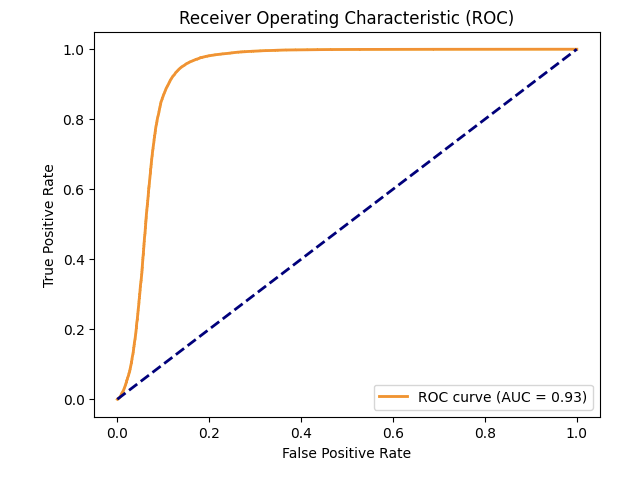
\includegraphics[width=\textwidth]{figures/model/bad_roc.jpg}
        \caption{ROC Curve from Logistic Regression.}
        \label{fig:bad_roc}
    \end{minipage} \hfill
    \begin{minipage}{0.48\textwidth}
        \centering
        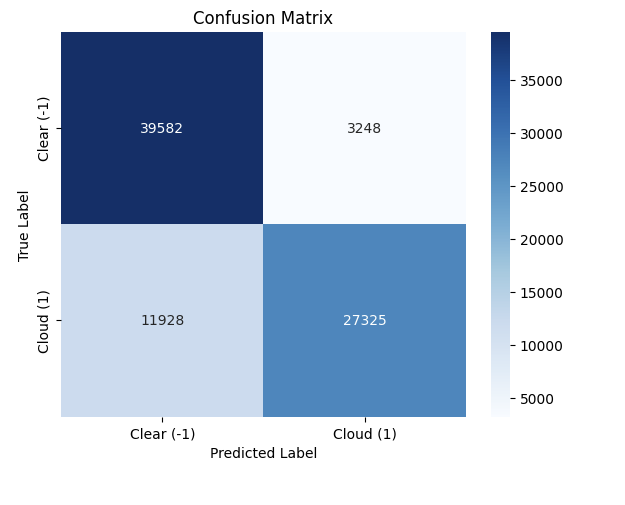
\includegraphics[width=\textwidth]{figures/model/bad_confusion.jpg}
        \caption{Confusion Matrix from Logistic Regression.}
        \label{fig:bad_confusion}
    \end{minipage}
\end{figure}

The permutation feature importance analysis (Figure \ref{fig:perm_importance}) reveals that \texttt{SD} is the most dominant feature. The confusion matrix (Figure \ref{fig:confusion_matrix}) shows that the model is particularly strong at identifying clouds (Recall = 0.9950). 

\begin{figure}[H]
    \centering
    \begin{minipage}{0.48\textwidth}
        \centering
        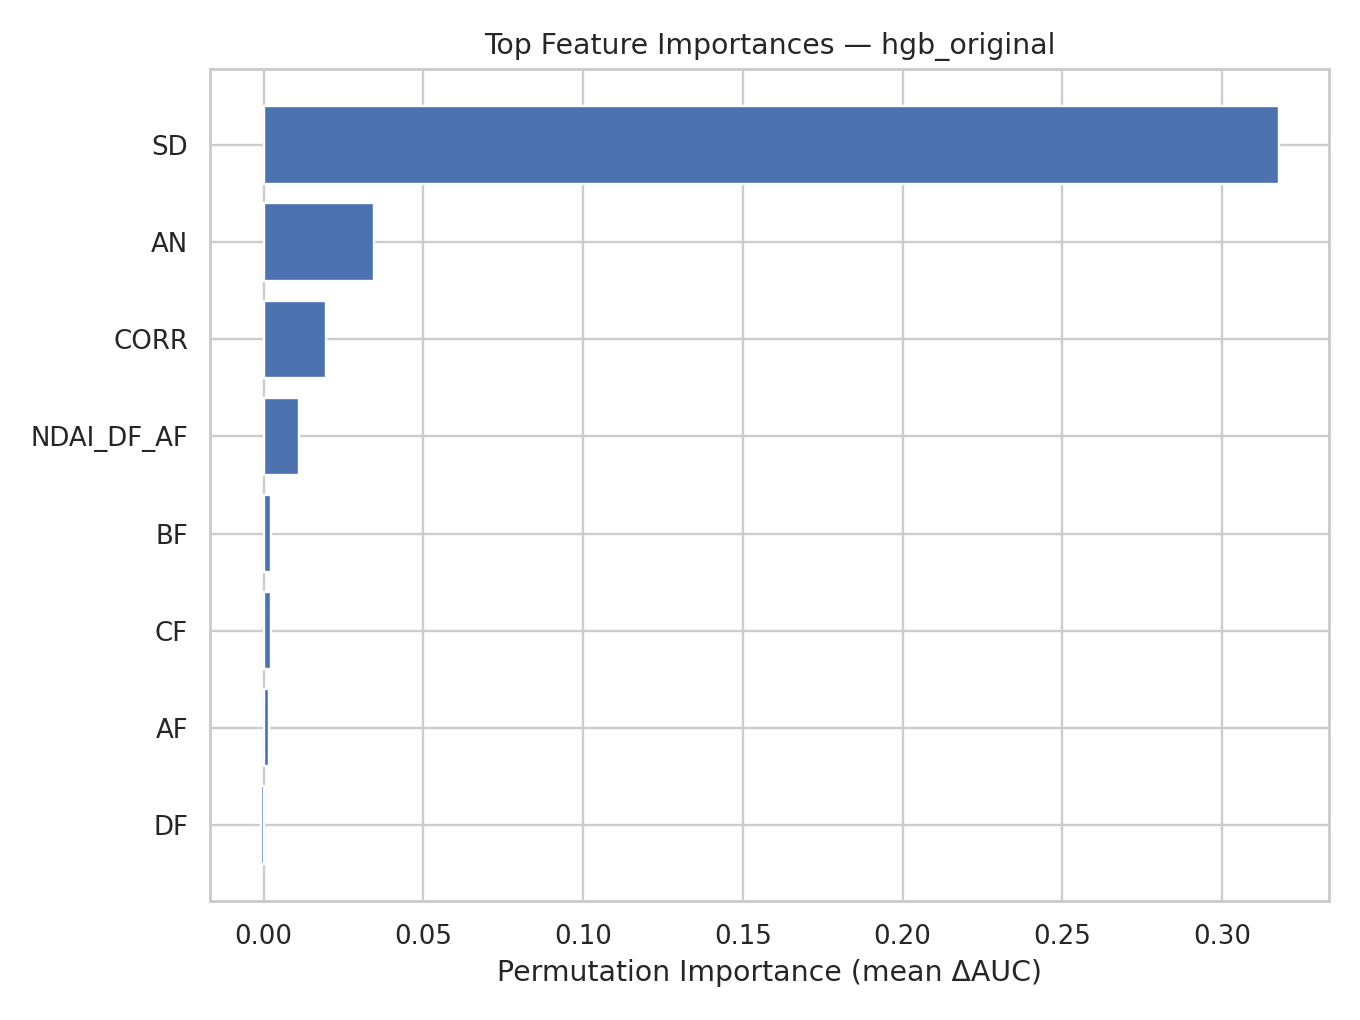
\includegraphics[width=\textwidth]{figures/model/fig_model_hgb_permutation_importance.png}
        \caption{Top features by permutation importance for the HGB model.}
        \label{fig:perm_importance}
    \end{minipage} \hfill
    \begin{minipage}{0.48\textwidth}
        \centering
        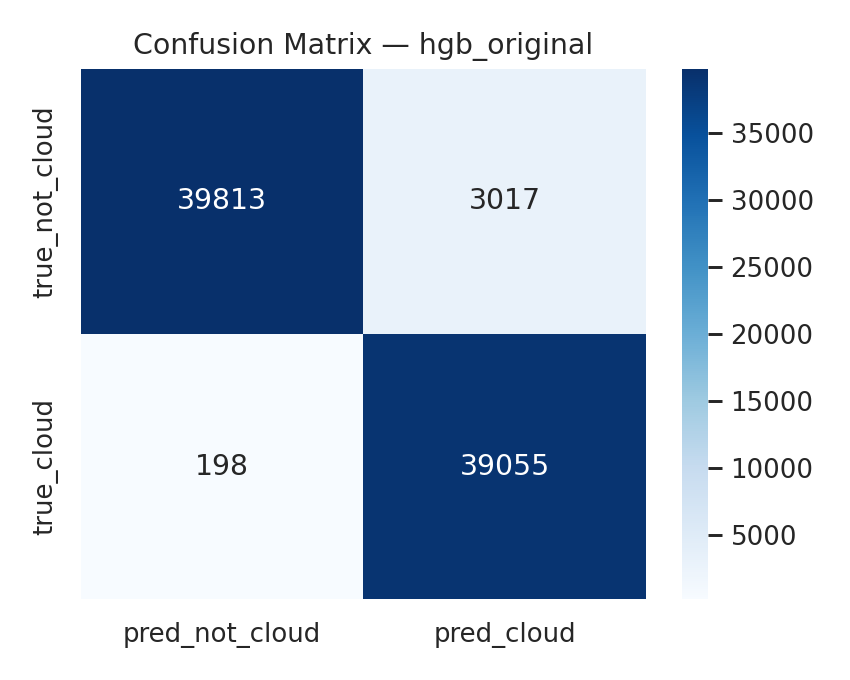
\includegraphics[width=\textwidth]{figures/model/fig_model_hgb_confusion_matrix.png}
        \caption{Confusion matrix for HGB on the temporal holdout set.}
        \label{fig:confusion_matrix}
    \end{minipage}
\end{figure}

\subsection{Post-hoc Error EDA and Boundary Analysis}
Spatial visualization of misclassifications (Figure \ref{fig:spatial_errors}) reveals that errors cluster at the boundaries of clouds. To quantify this effect, we calculated the Euclidean distance from each pixel to the nearest pixel of the opposite class (the ``label boundary"). 

While the theoretical minimum distance between adjacent grid pixels is 1.0 unit, our analysis of the temporal holdout set (\texttt{O013490}) revealed an empirical minimum distance of \textbf{6.0} units between labeled pixels of opposite classes. This indicates a spatial buffer or a lower-resolution sampling in the expert-provided labels for this orbit.

Despite this labeling gap, the quantitative trend (Figure \ref{fig:boundary_error}) is clear: the error rate spikes to $\approx 50\%$ at this observable 6-unit threshold and decays rapidly to $<1\%$ for pixels located more than 100 units from a transition. This confirms that the model's uncertainty is almost entirely localized at spatial boundaries.


Presumably out of the same reason, similar location patterns appear in spatial distribution of misclassified data points in SVM model (Figure \ref{fig:svm_spatial}). With a lower accuracy, Logistic Regression Model is not able to capture a piece of cloud in the middle of the graph, reflecting lack of further information retrieval from selected features (Figure \ref{fig:logreg_spatial}).


\begin{figure}[H]
    \centering
    \begin{minipage}{0.48\textwidth}
        \centering
        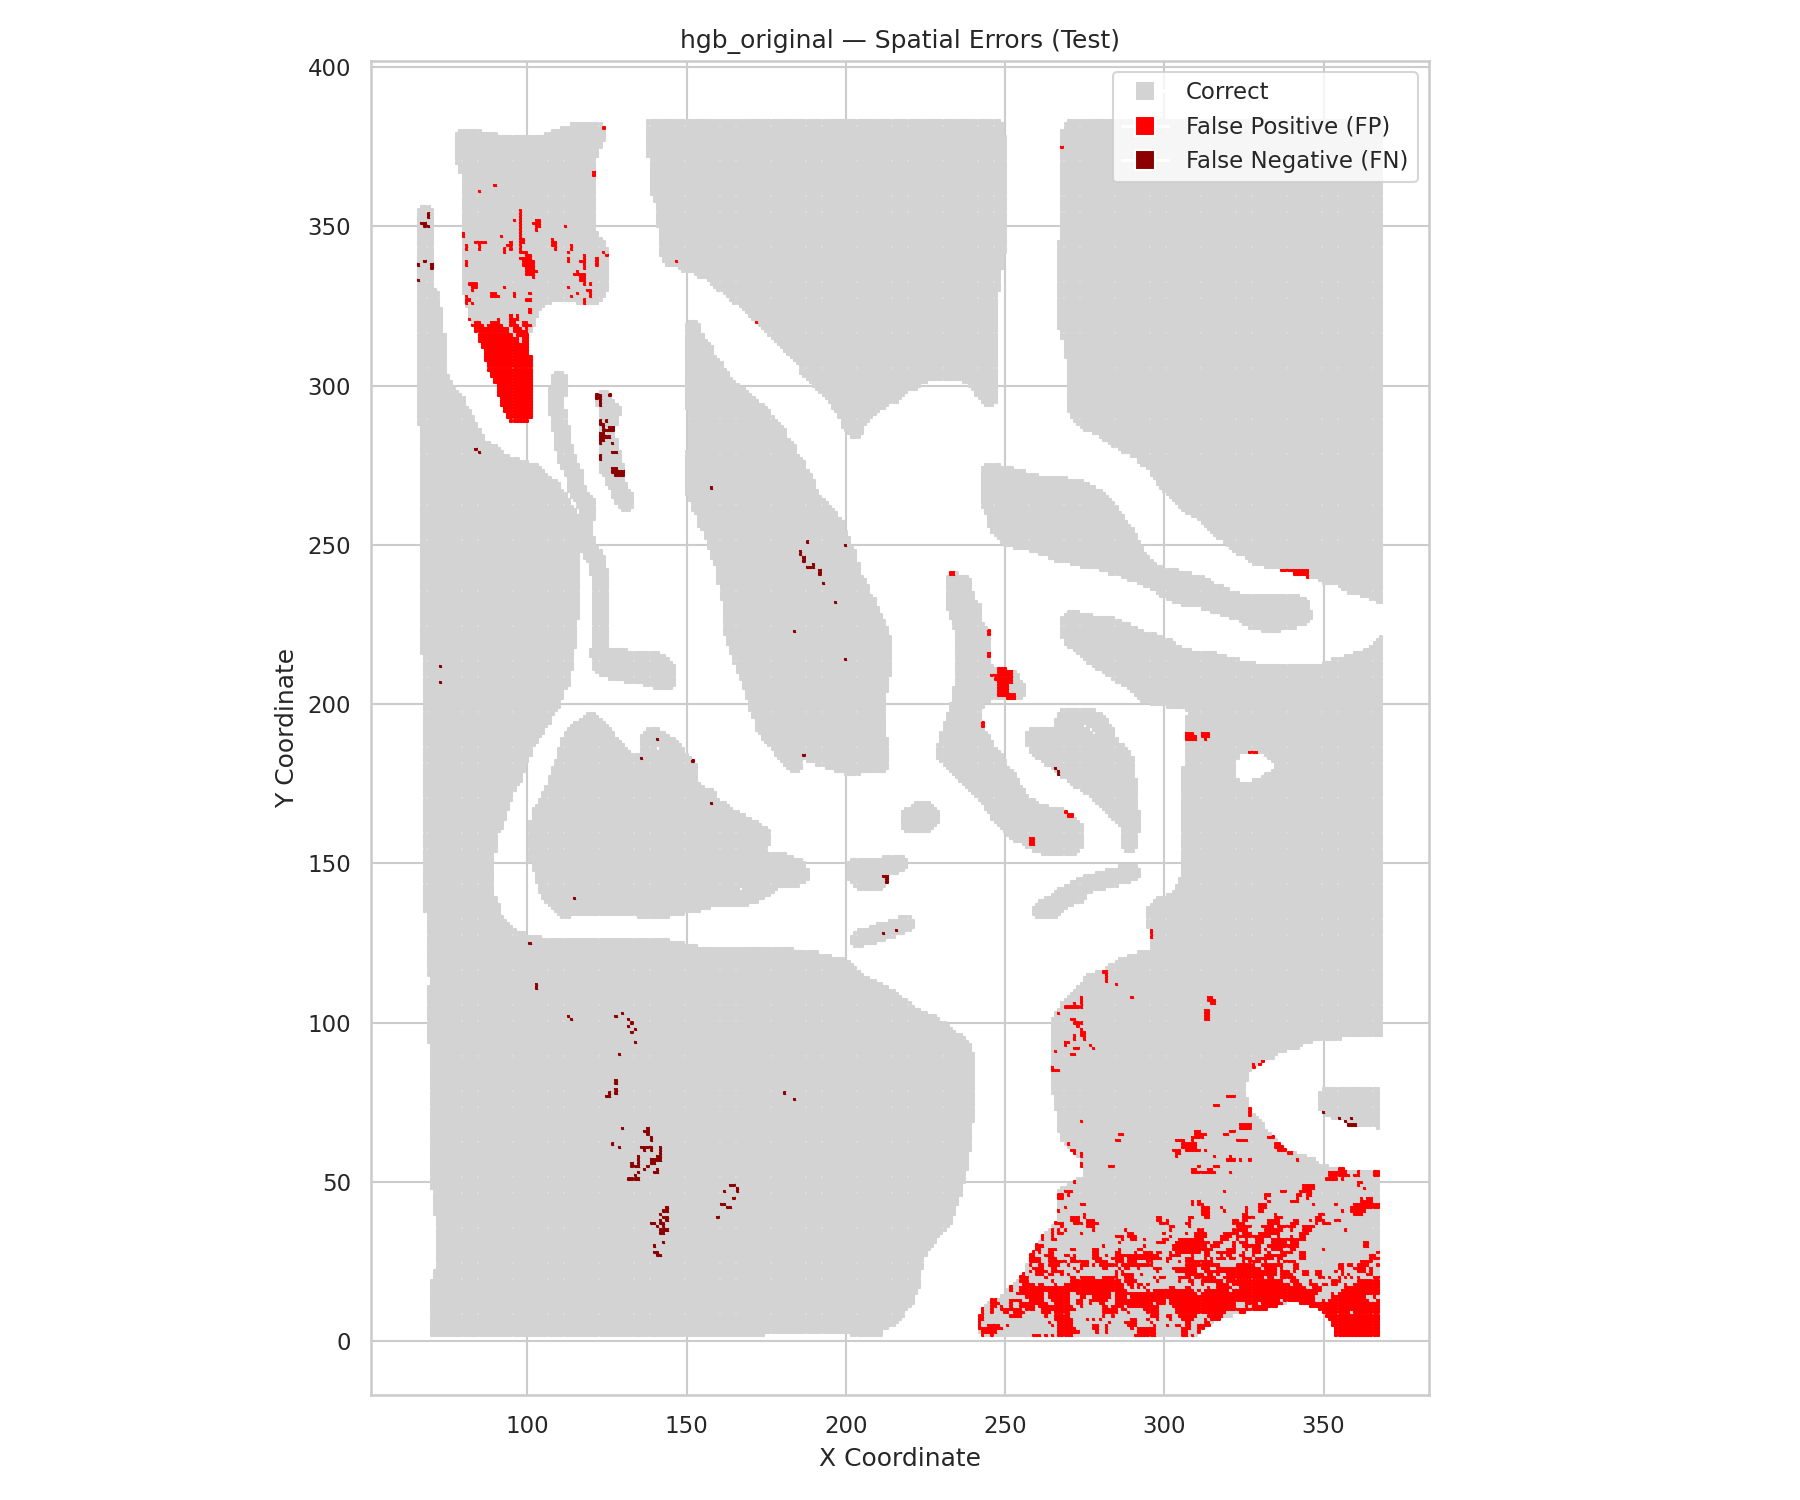
\includegraphics[width=0.9\textwidth]{figures/model/fig_model_hgb_spatial_errors.png}
        \caption{Spatial map of classification errors concentrated at cloud edges.}
        \label{fig:spatial_errors}
    \end{minipage} \hfill
    \begin{minipage}{0.48\textwidth}
        \centering
        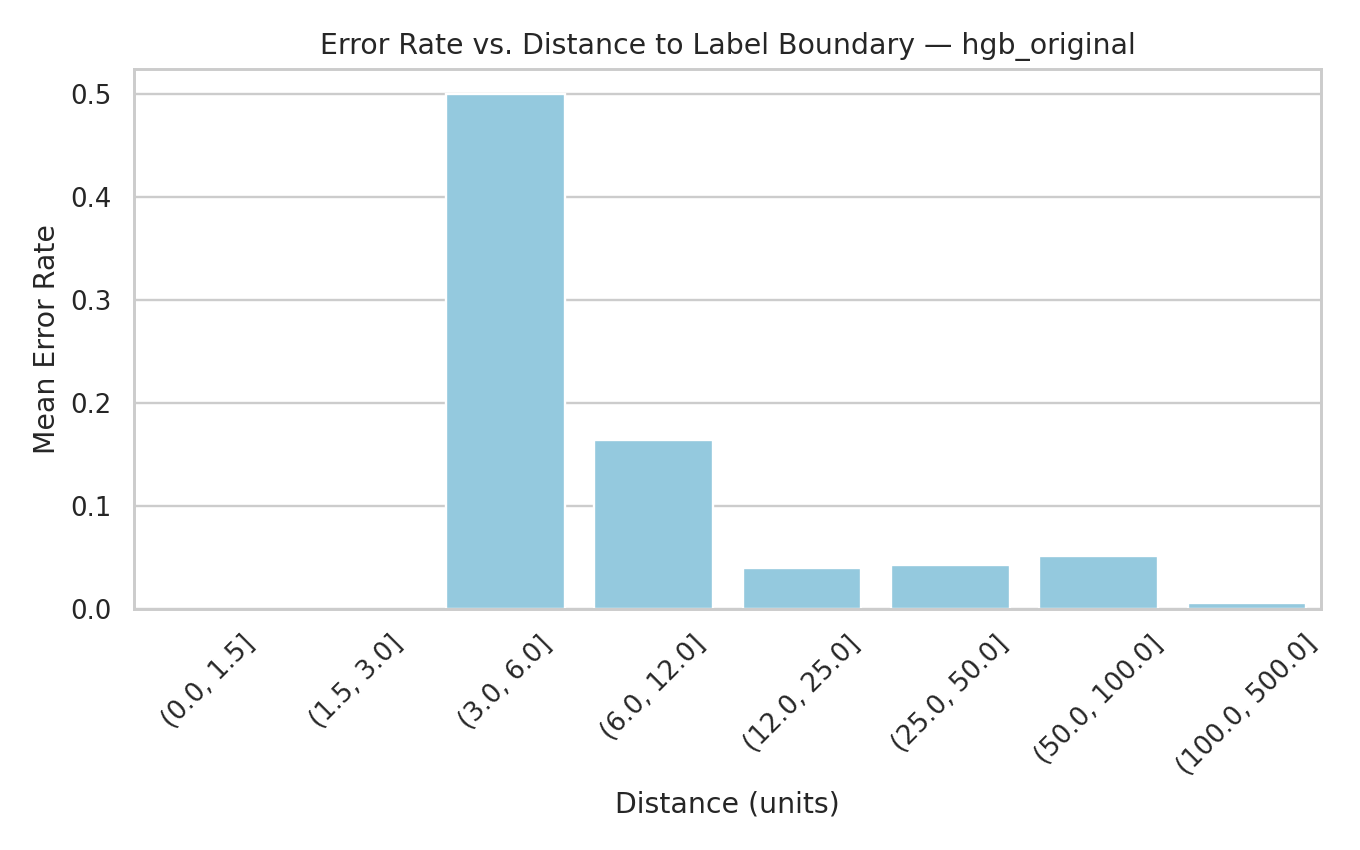
\includegraphics[width=\textwidth]{figures/model/fig_model_hgb_boundary_error.png}
        \caption{Mean Error Rate vs. Distance to Label Boundary.}
        \label{fig:boundary_error}
    \end{minipage}
\end{figure}
% \begin{figure}[H]
%     \centering
%     \begin{minipage}{0.48\textwidth}
%         \centering
%         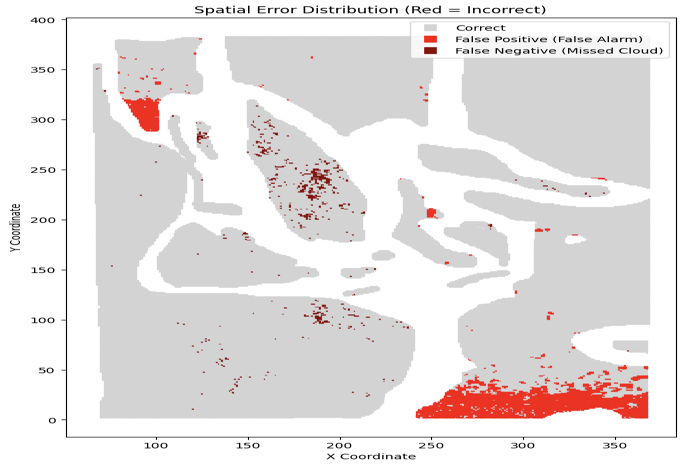
\includegraphics[width=\textwidth]{figures/model/svm_spatial.jpg}
%         \caption{Spatial map of classification errors in SVM(Lit) model setting.}
%         \label{fig:svm_spatial}
%     \end{minipage} \hfill
%     \begin{minipage}{0.48\textwidth}
%         \centering
%         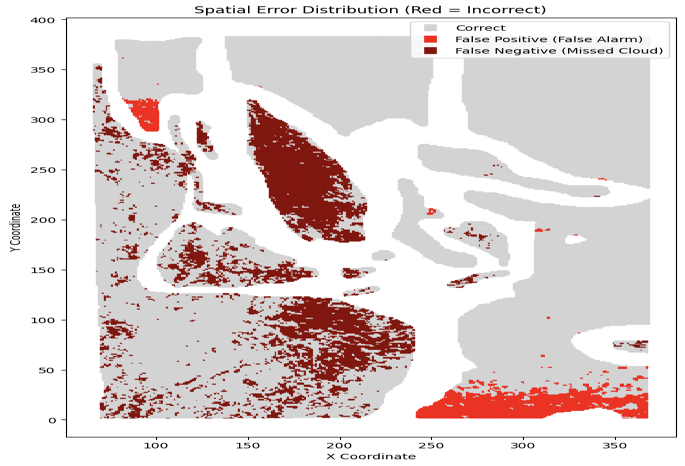
\includegraphics[width=\textwidth]{figures/model/logreg_spatial.jpg}
%         \caption{Spatial map of classification errors in Stepwise Logistic Regression.}
%         \label{fig:logreg_spatial}
%     \end{minipage}
% \end{figure}
\begin{figure}[H]
    \centering

    \begin{minipage}[t]{0.48\textwidth}
        \centering
        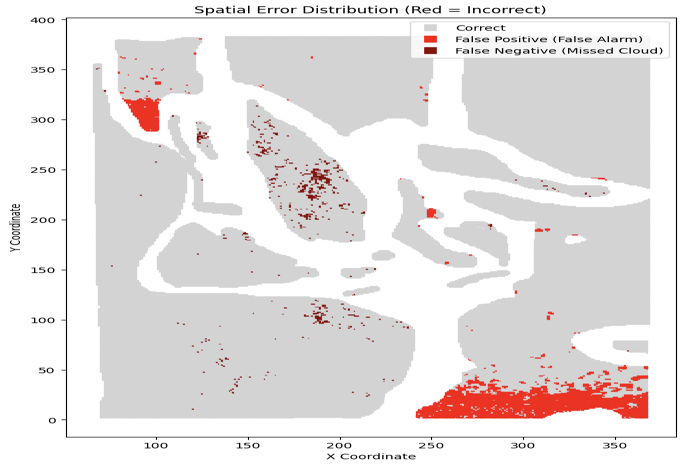
\includegraphics[width=0.6\textwidth,height=6cm]{figures/model/svm_spatial.jpg}
        \caption{Spatial map of classification errors in the SVM (Lit) model setting.}
        \label{fig:svm_spatial}
    \end{minipage}
    \hfill
    \begin{minipage}[t]{0.48\textwidth}
        \centering
        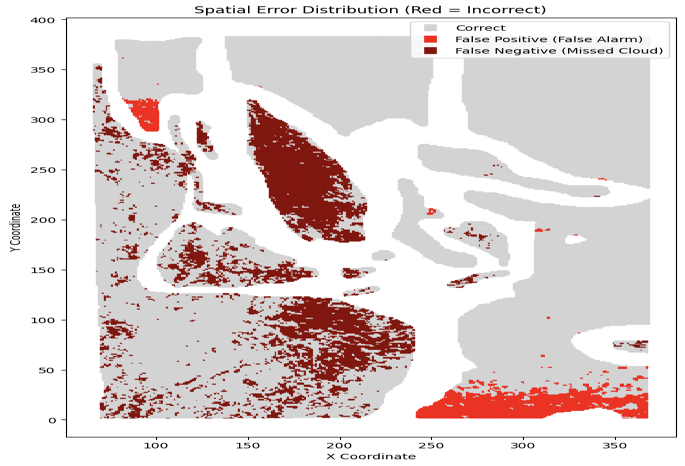
\includegraphics[width=0.6\textwidth,height=6cm]{figures/model/logreg_spatial.jpg}
        \caption{Spatial map of classification errors in the Stepwise Logistic Regression model.}
        \label{fig:logreg_spatial}
    \end{minipage}

\end{figure}

Additionally, the diagnostic assessment of the SVM model was conducted by employing PCA to visualize both the decision clusters and the support vector density in a reduced-dimensional space (Figure \ref{fig:svm_pca}). The results of this projection demonstrate a high degree of internal consistency. Specifically, a visible double peak emerges within the two-dimensional principal component space, characterized by support vectors distributed strategically along the decision boundaries to separate the two binary classes. This spatial arrangement confirms that the model has identified a stable structural manifold for classification.
\begin{figure}[H]
    \centering
    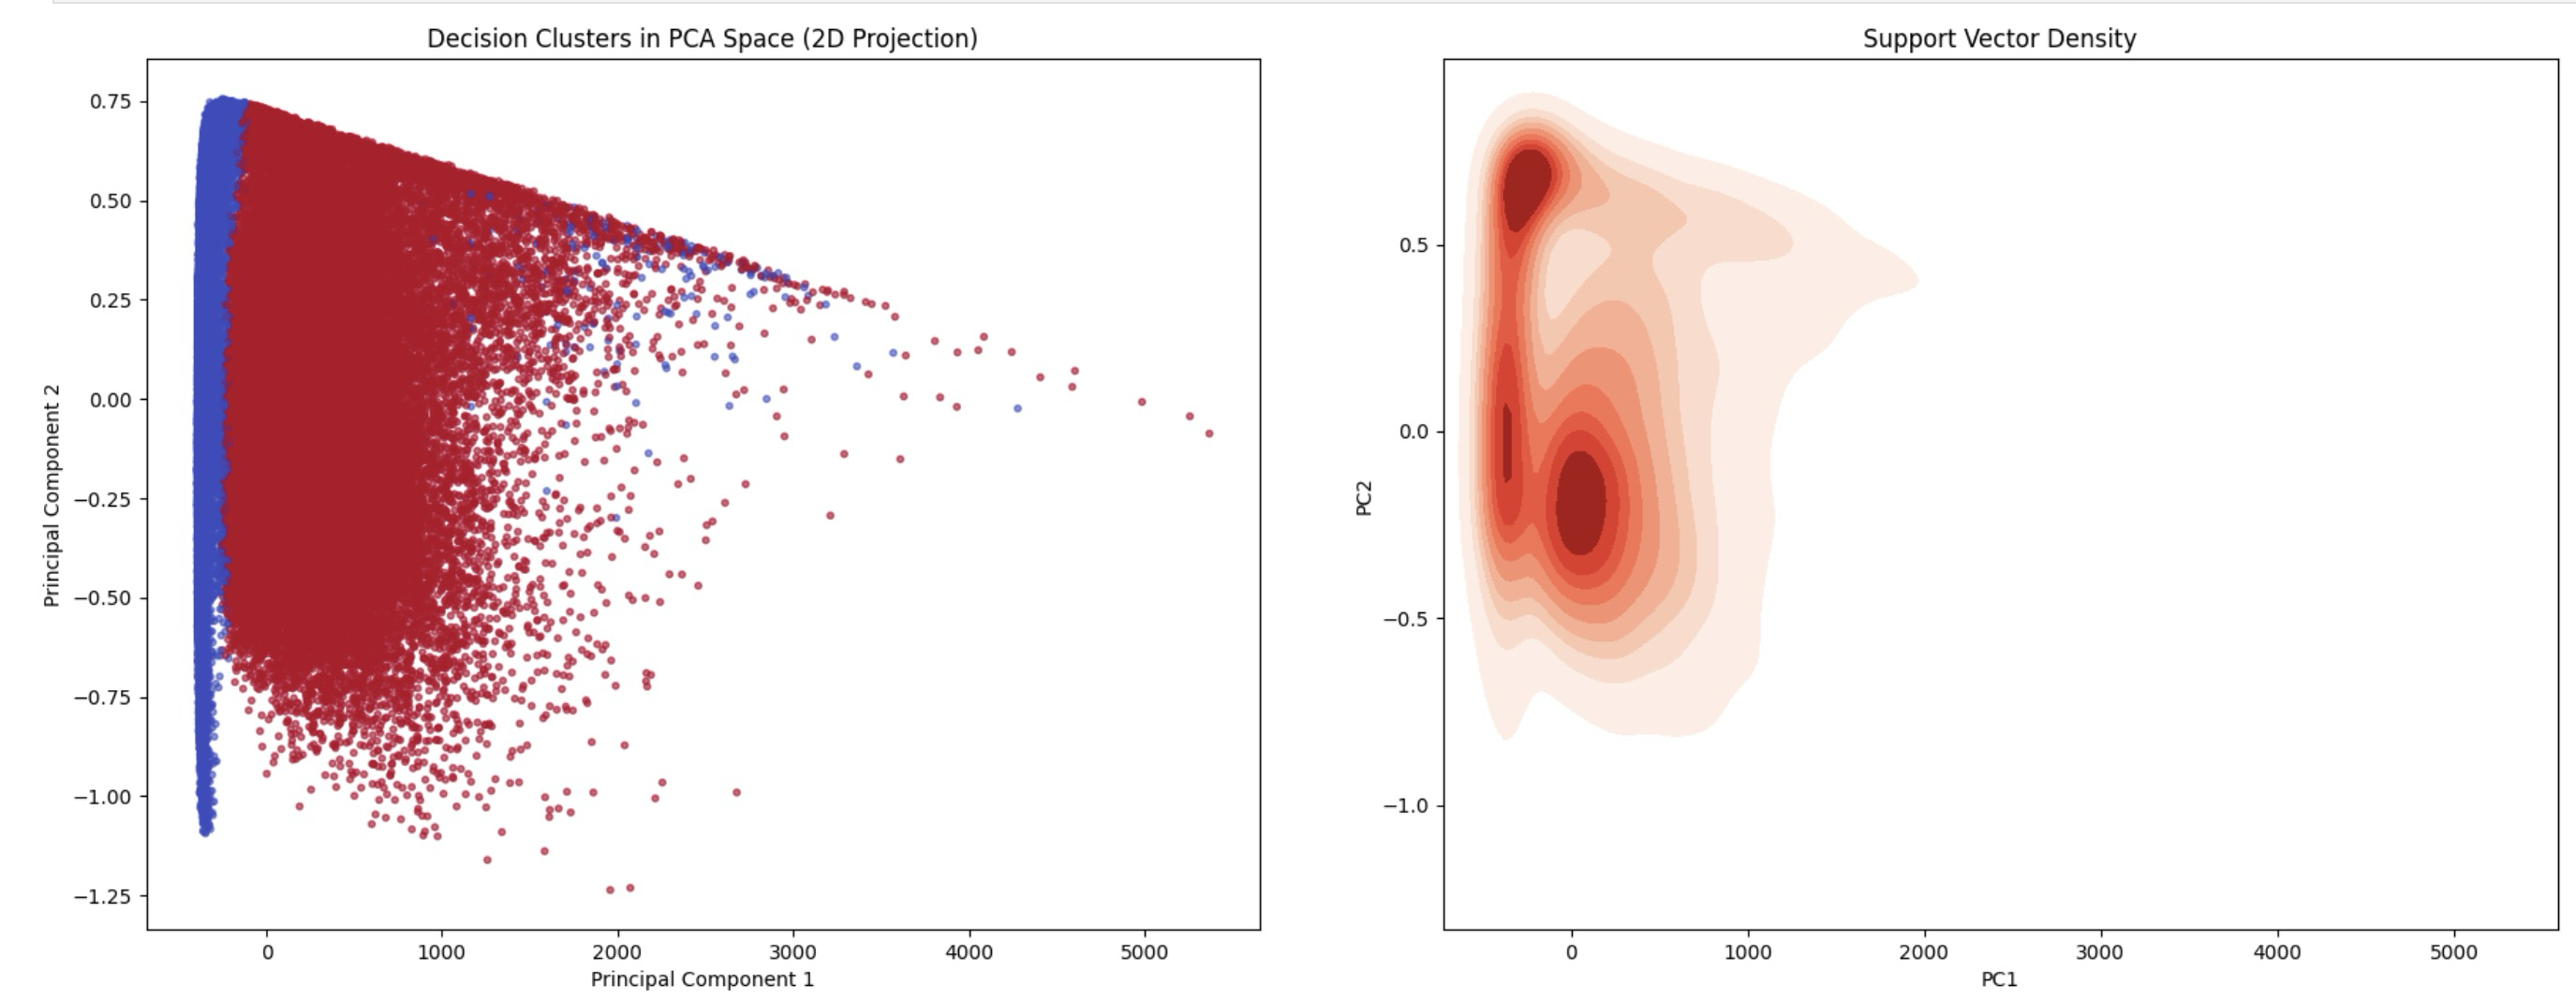
\includegraphics[width=0.9\textwidth]{figures/model/pca_svm.jpg}
    \caption{PCA visualizations of both the decision clusters and the support vector density into 2 dimensions. Visible trend of double peaks are coherent with the robust performance of the SVM model.}
    \label{fig:svm_pca}
\end{figure}

For non-ensemble learning models, the primary change would be collinearity and overfitting. Lasso Logistic Regression and SVM seem to be severely influenced by the difference of features included. With SVM, the best model included only three features in the model \texttt{SD}, \texttt{CORR}, and \texttt{NDAI}. As seen from model metrics discussed above (Figure \ref{tab:model_comparison}), adding one additional feature into the predictors (the first \texttt{PC}, for example) will immediately compromise the accuracy score on the test set down to approximately 0.4. In other words, even with non-linear kernel function, additional dimensionality in predictors will bring radical change to the performance of SVM. Similarly, the features selected by Lasso regression include 7 variables, which has 2 more compared to the best performance given by stepwise regression, the corresponding collinearity problem already reflected in the fit assessment. By constraining the complexity of the feature space and regularizing the optimization objectives, the models are better equipped to generalize beyond the training data. 

Investigation into the features driving these boundary errors revealed a significant shift in \texttt{CORR} (correlation). The mean \texttt{CORR} for pixels near boundaries ($<15$ units) is \textbf{0.473}, compared to only \textbf{0.097} for pixels deep within homogeneous regions. This suggests that the high-frequency textures associated with cloud edges or fragmented cover are the primary challenge for the ensemble learning model, as they present feature signatures that are intermediate between clear sky and dense cloud.

We further analyzed the distributions of key features across four groups: True Negatives (TN), True Positives (TP), False Positives (FP), and False Negatives (FN). The statistical summaries (Table \ref{tab:error_group_stats}) and distributions (Figure \ref{fig:error_violins}) reveal distinct feature signatures for misclassifications.

\begin{table}[H]
\centering
\begin{tabular}{llcccc}
\toprule
\textbf{Feature} & \textbf{Metric} & \textbf{TN} & \textbf{TP} & \textbf{FP} & \textbf{FN} \\ 
\midrule
\texttt{SD}   & Mean   & 89.82  & 705.98 & 773.81  & \textbf{1376.21} \\
              & Median & 37.39  & 619.14 & 622.54  & \textbf{1032.57} \\
\midrule
\texttt{CORR} & Mean   & 0.263  & 0.196  & \textbf{0.823}   & 0.667 \\
              & Median & 0.230  & 0.161  & \textbf{0.909}   & 0.791 \\
\midrule
\texttt{NDAI} & Mean   & 0.109  & 0.299  & 0.177   & 0.235 \\
              & Median & 0.103  & 0.262  & 0.182   & 0.205 \\
\bottomrule
\end{tabular}
\caption{Feature distribution statistics by classification group. High \texttt{SD} drives missed clouds (FN), while high \texttt{CORR} is the primary driver of false clouds (FP).}
\label{tab:error_group_stats}
\end{table}

\begin{figure}[H]
    \centering
    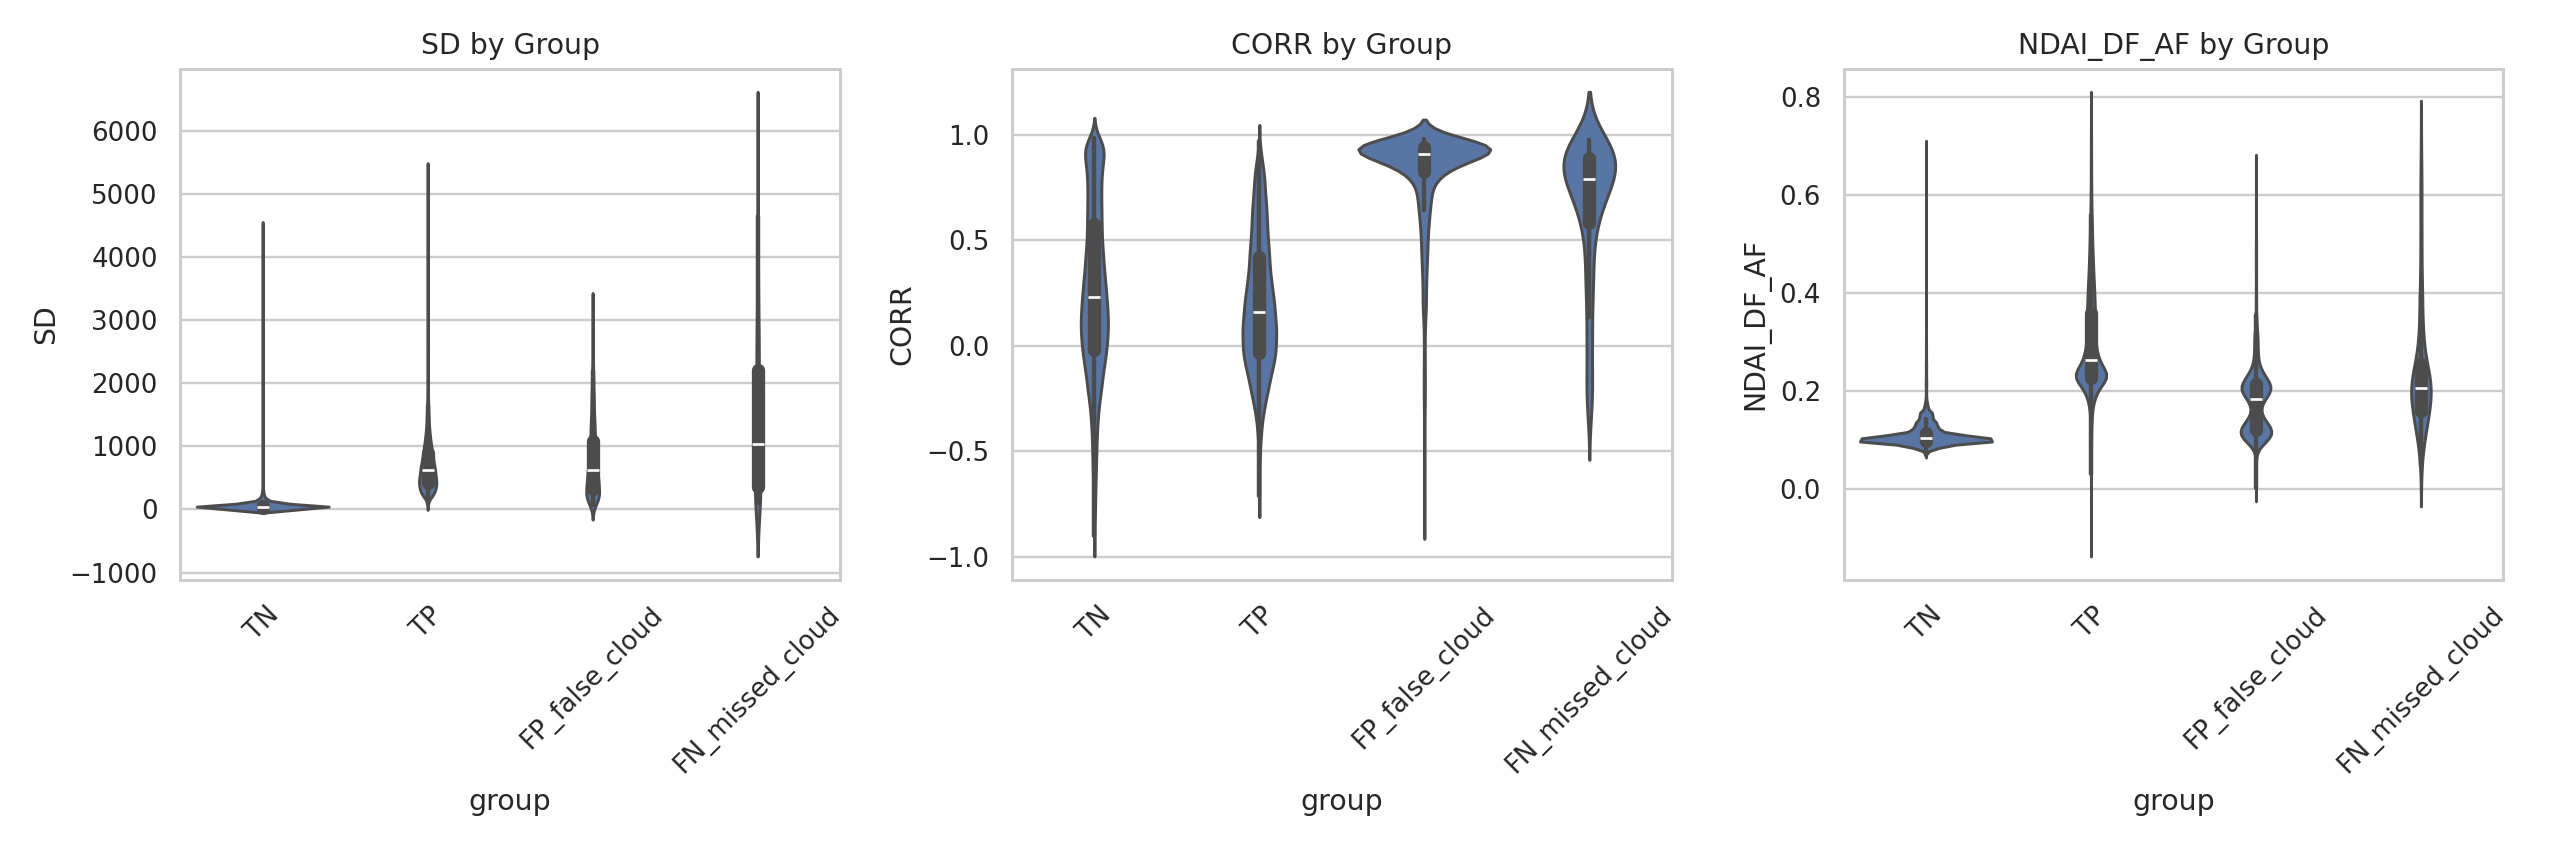
\includegraphics[width=\textwidth]{figures/model/fig_model_hgb_error_group_violins.png}
    \caption{Violin plots of feature distributions across classification groups. Missed clouds (FN) are characterized by extreme spatial deviation (SD), whereas false clouds (FP) show exceptionally high correlation (CORR).}
    \label{fig:error_violins}
\end{figure}

The analysis indicates two primary failure modes:
\begin{enumerate}
    \item \textbf{Texture-Driven False Negatives:} The missed clouds (FN) exhibit substantially higher \texttt{SD} values (mean 1376.2) than the correctly identified clouds. This suggests that the model fails to detect clouds in regions of extreme heterogeneity or high-frequency surface features, where the cloud signal is "masked" by spatial complexity.
    \item \textbf{Correlation-Driven False Positives:} False clouds (FP) are strongly associated with extremely high \texttt{CORR} values (median 0.909). These high correlation signatures likely arise from smooth clear-sky surfaces (e.g., ice or water at specific angles) that mimic the smoothness typically associated with cloud layers, leading the model to overestimate cloud probability.
\end{enumerate}

\subsection{Stability and Future-Data Readiness}

\subsubsection{Predictions on Unlabeled Pixels}
Expert labelers assigned $\mathtt{label} = 0$ to pixels that were ambiguous at the time of annotation. For the 32,949 unlabeled pixels from orbit \texttt{O013490}, we applied the trained RF to these pixels to probe the model's behavior in the ambiguous regime.


The model classifies \textbf{82.7\%} (27,244) of unlabeled pixels as cloud and only 17.3\% (5,705) as non-cloud (Figure~\ref{fig:rf_unlabeled_map}). The probability histogram (Figure~\ref{fig:rf_unlabeled_hist}) 
shows a strongly bimodal distribution: most unlabeled pixels receive near-zero or near-one cloud probabilities, with relatively few landing in the $[0.3, 0.7]$ uncertain band.

\begin{figure}[H]
\centering

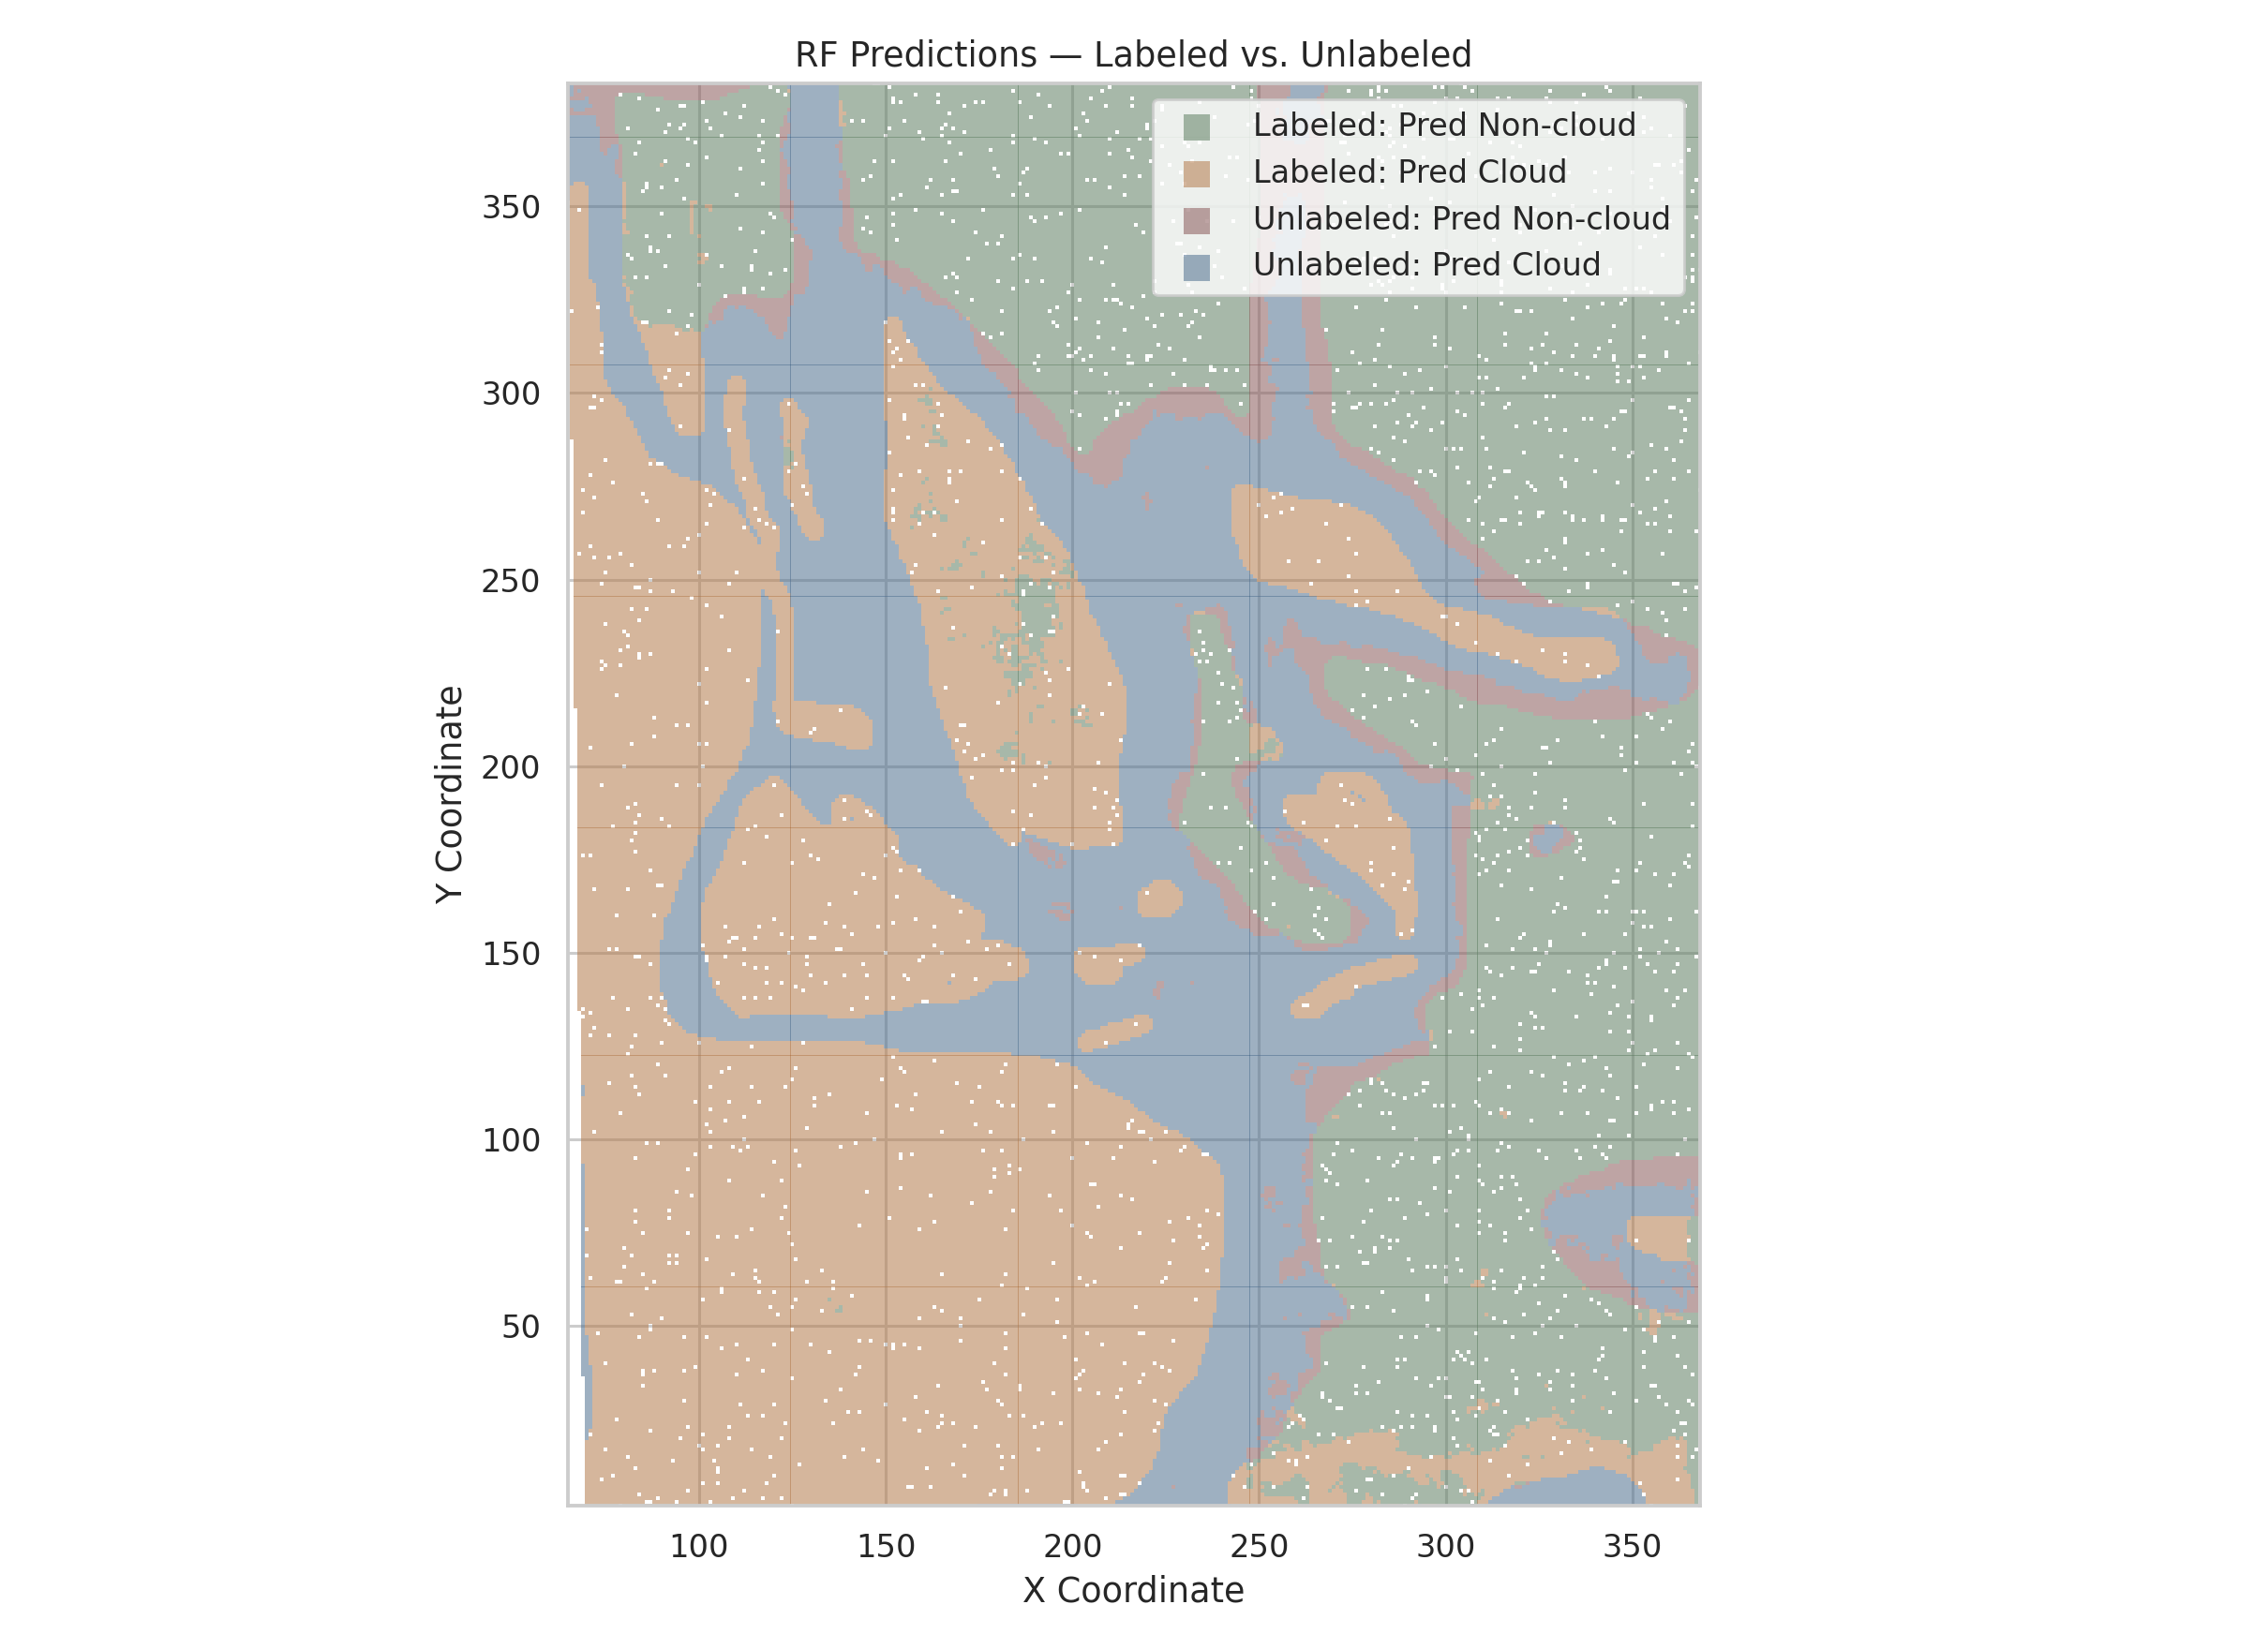
\includegraphics[width=0.9\textwidth]{figures/model/fig_model_rf_unlabeled_vs_labeled_spatial.png}
 \caption{Spatial map of orbit \texttt{O013490} showing RF predictions for all pixel types.}
\label{fig:rf_unlabeled_map}
\begin{minipage}{0.48\textwidth}
\centering
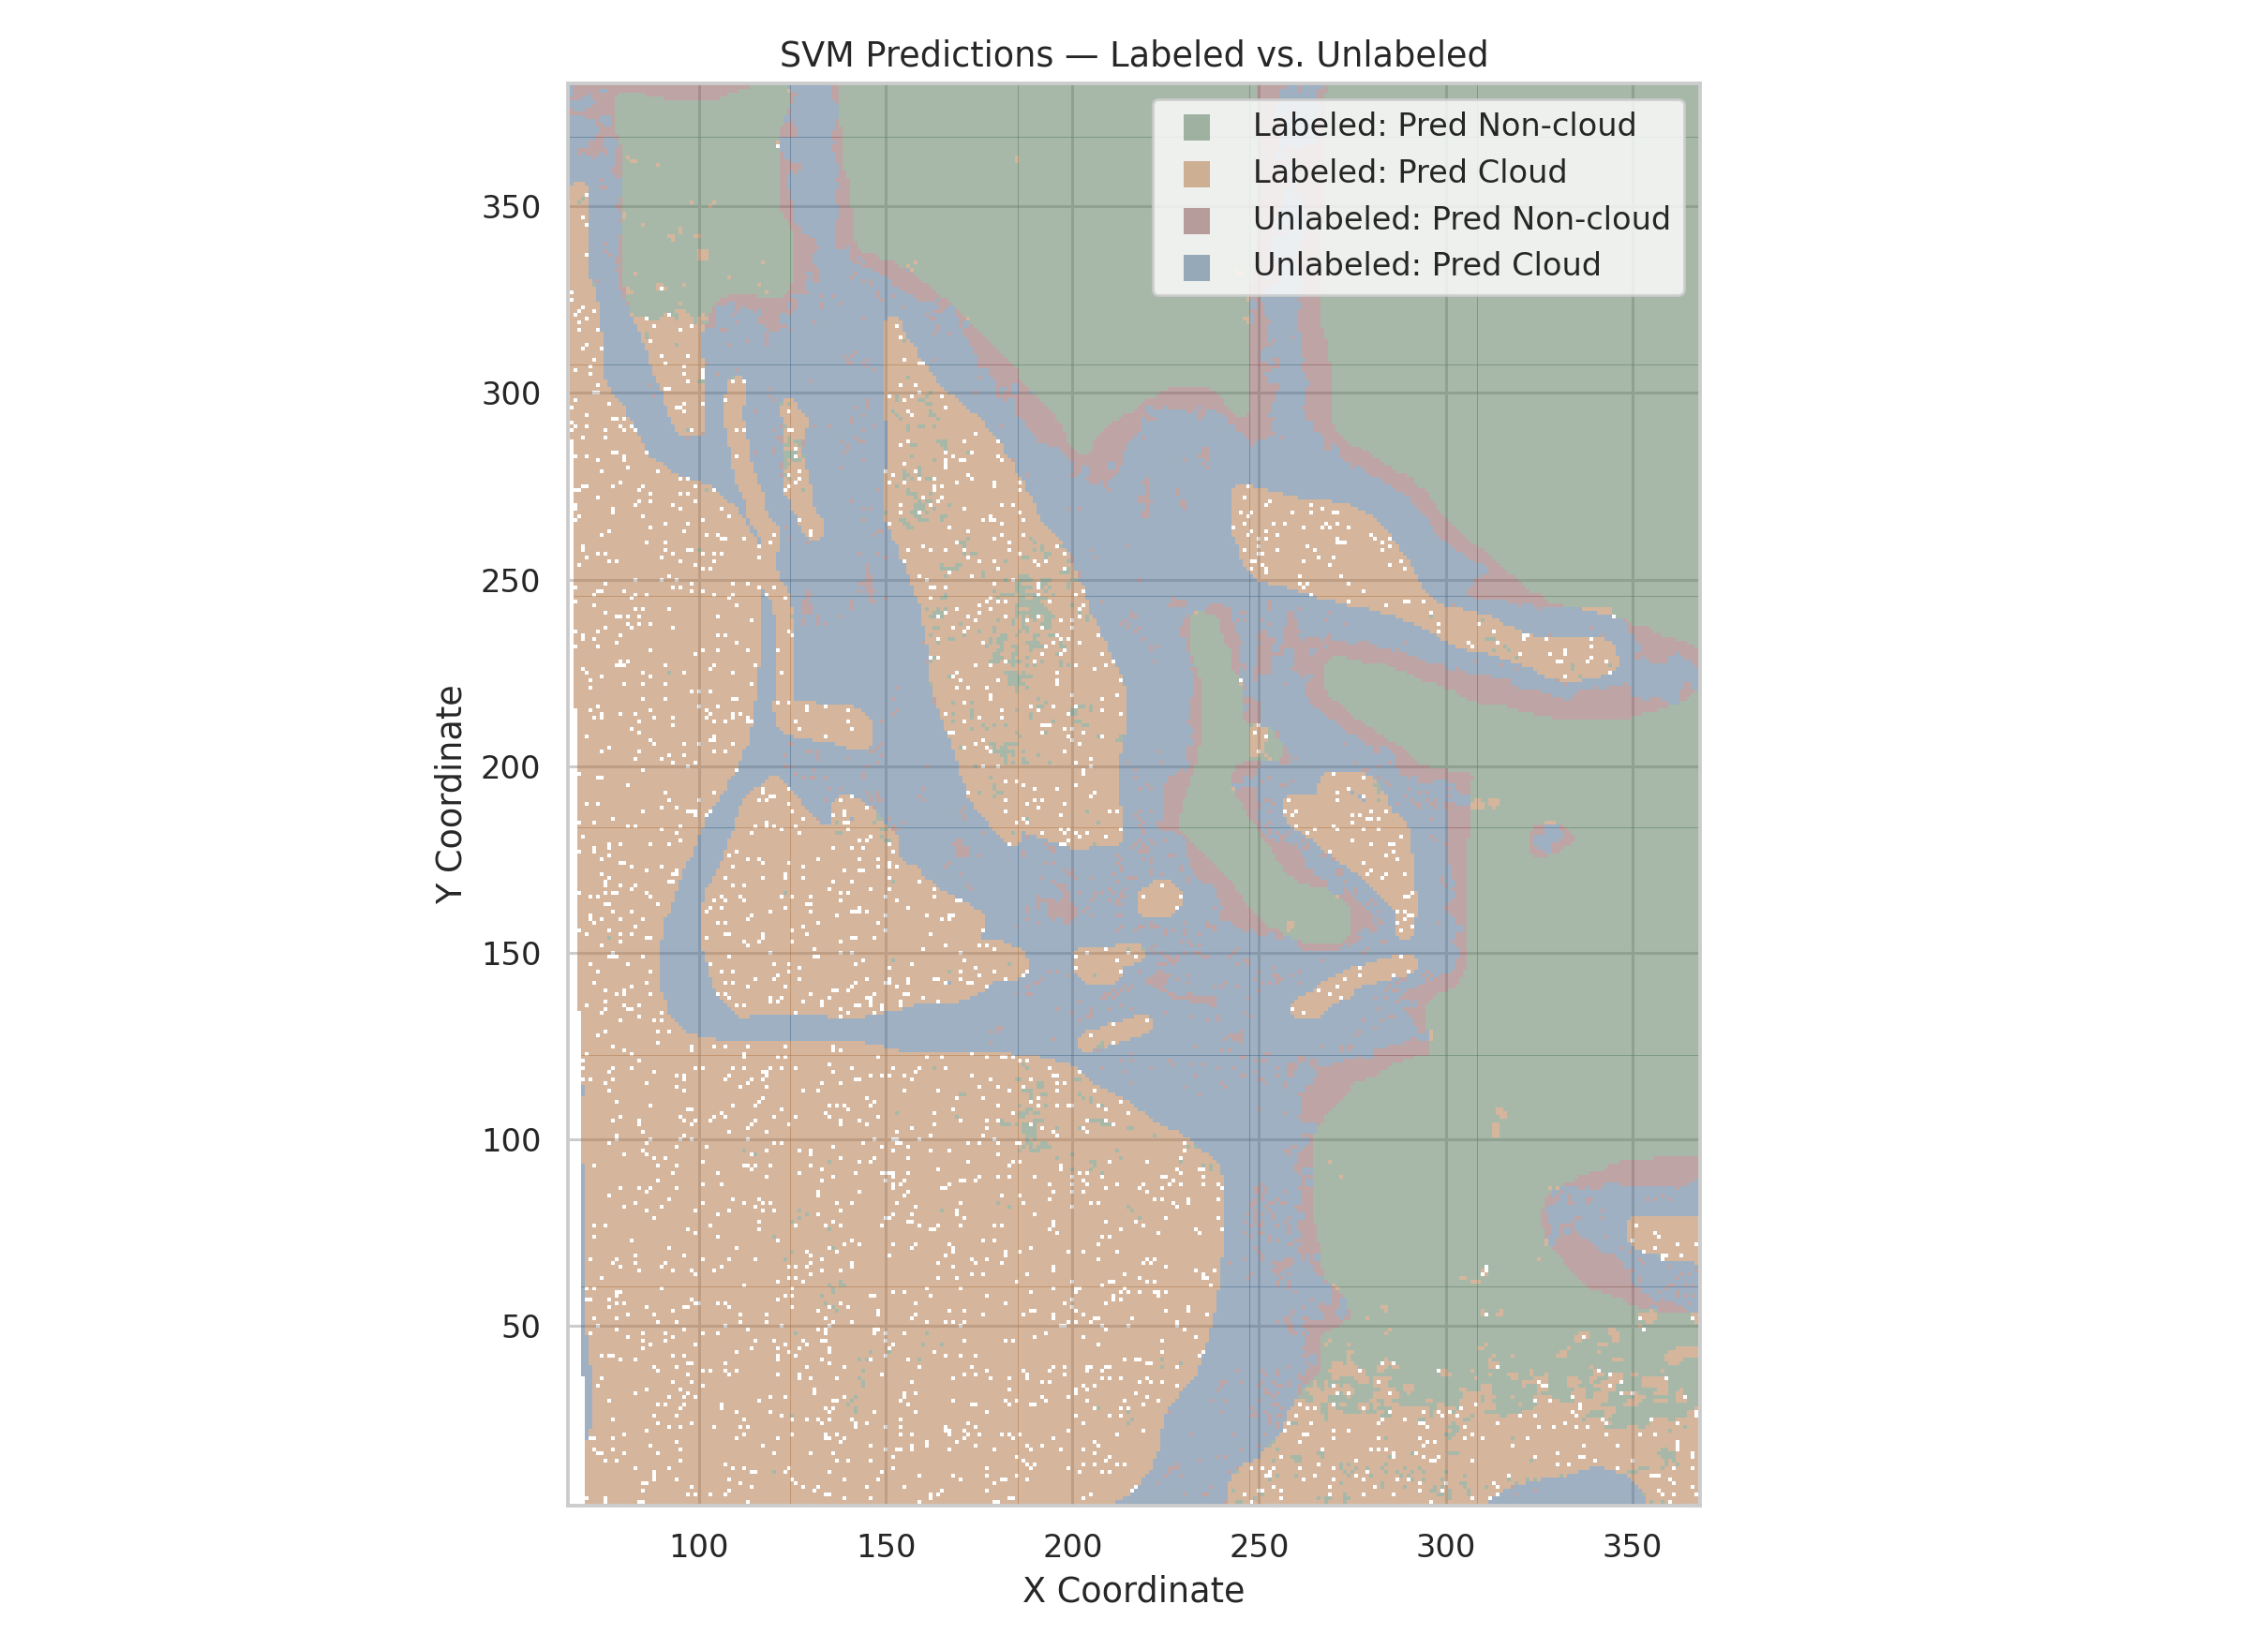
\includegraphics[width=\textwidth]{figures/model/svm_labeled_vs_unlabeled.png}
\caption{SVM spatial map}
\end{minipage}
\hfill
\begin{minipage}{0.48\textwidth}
\centering
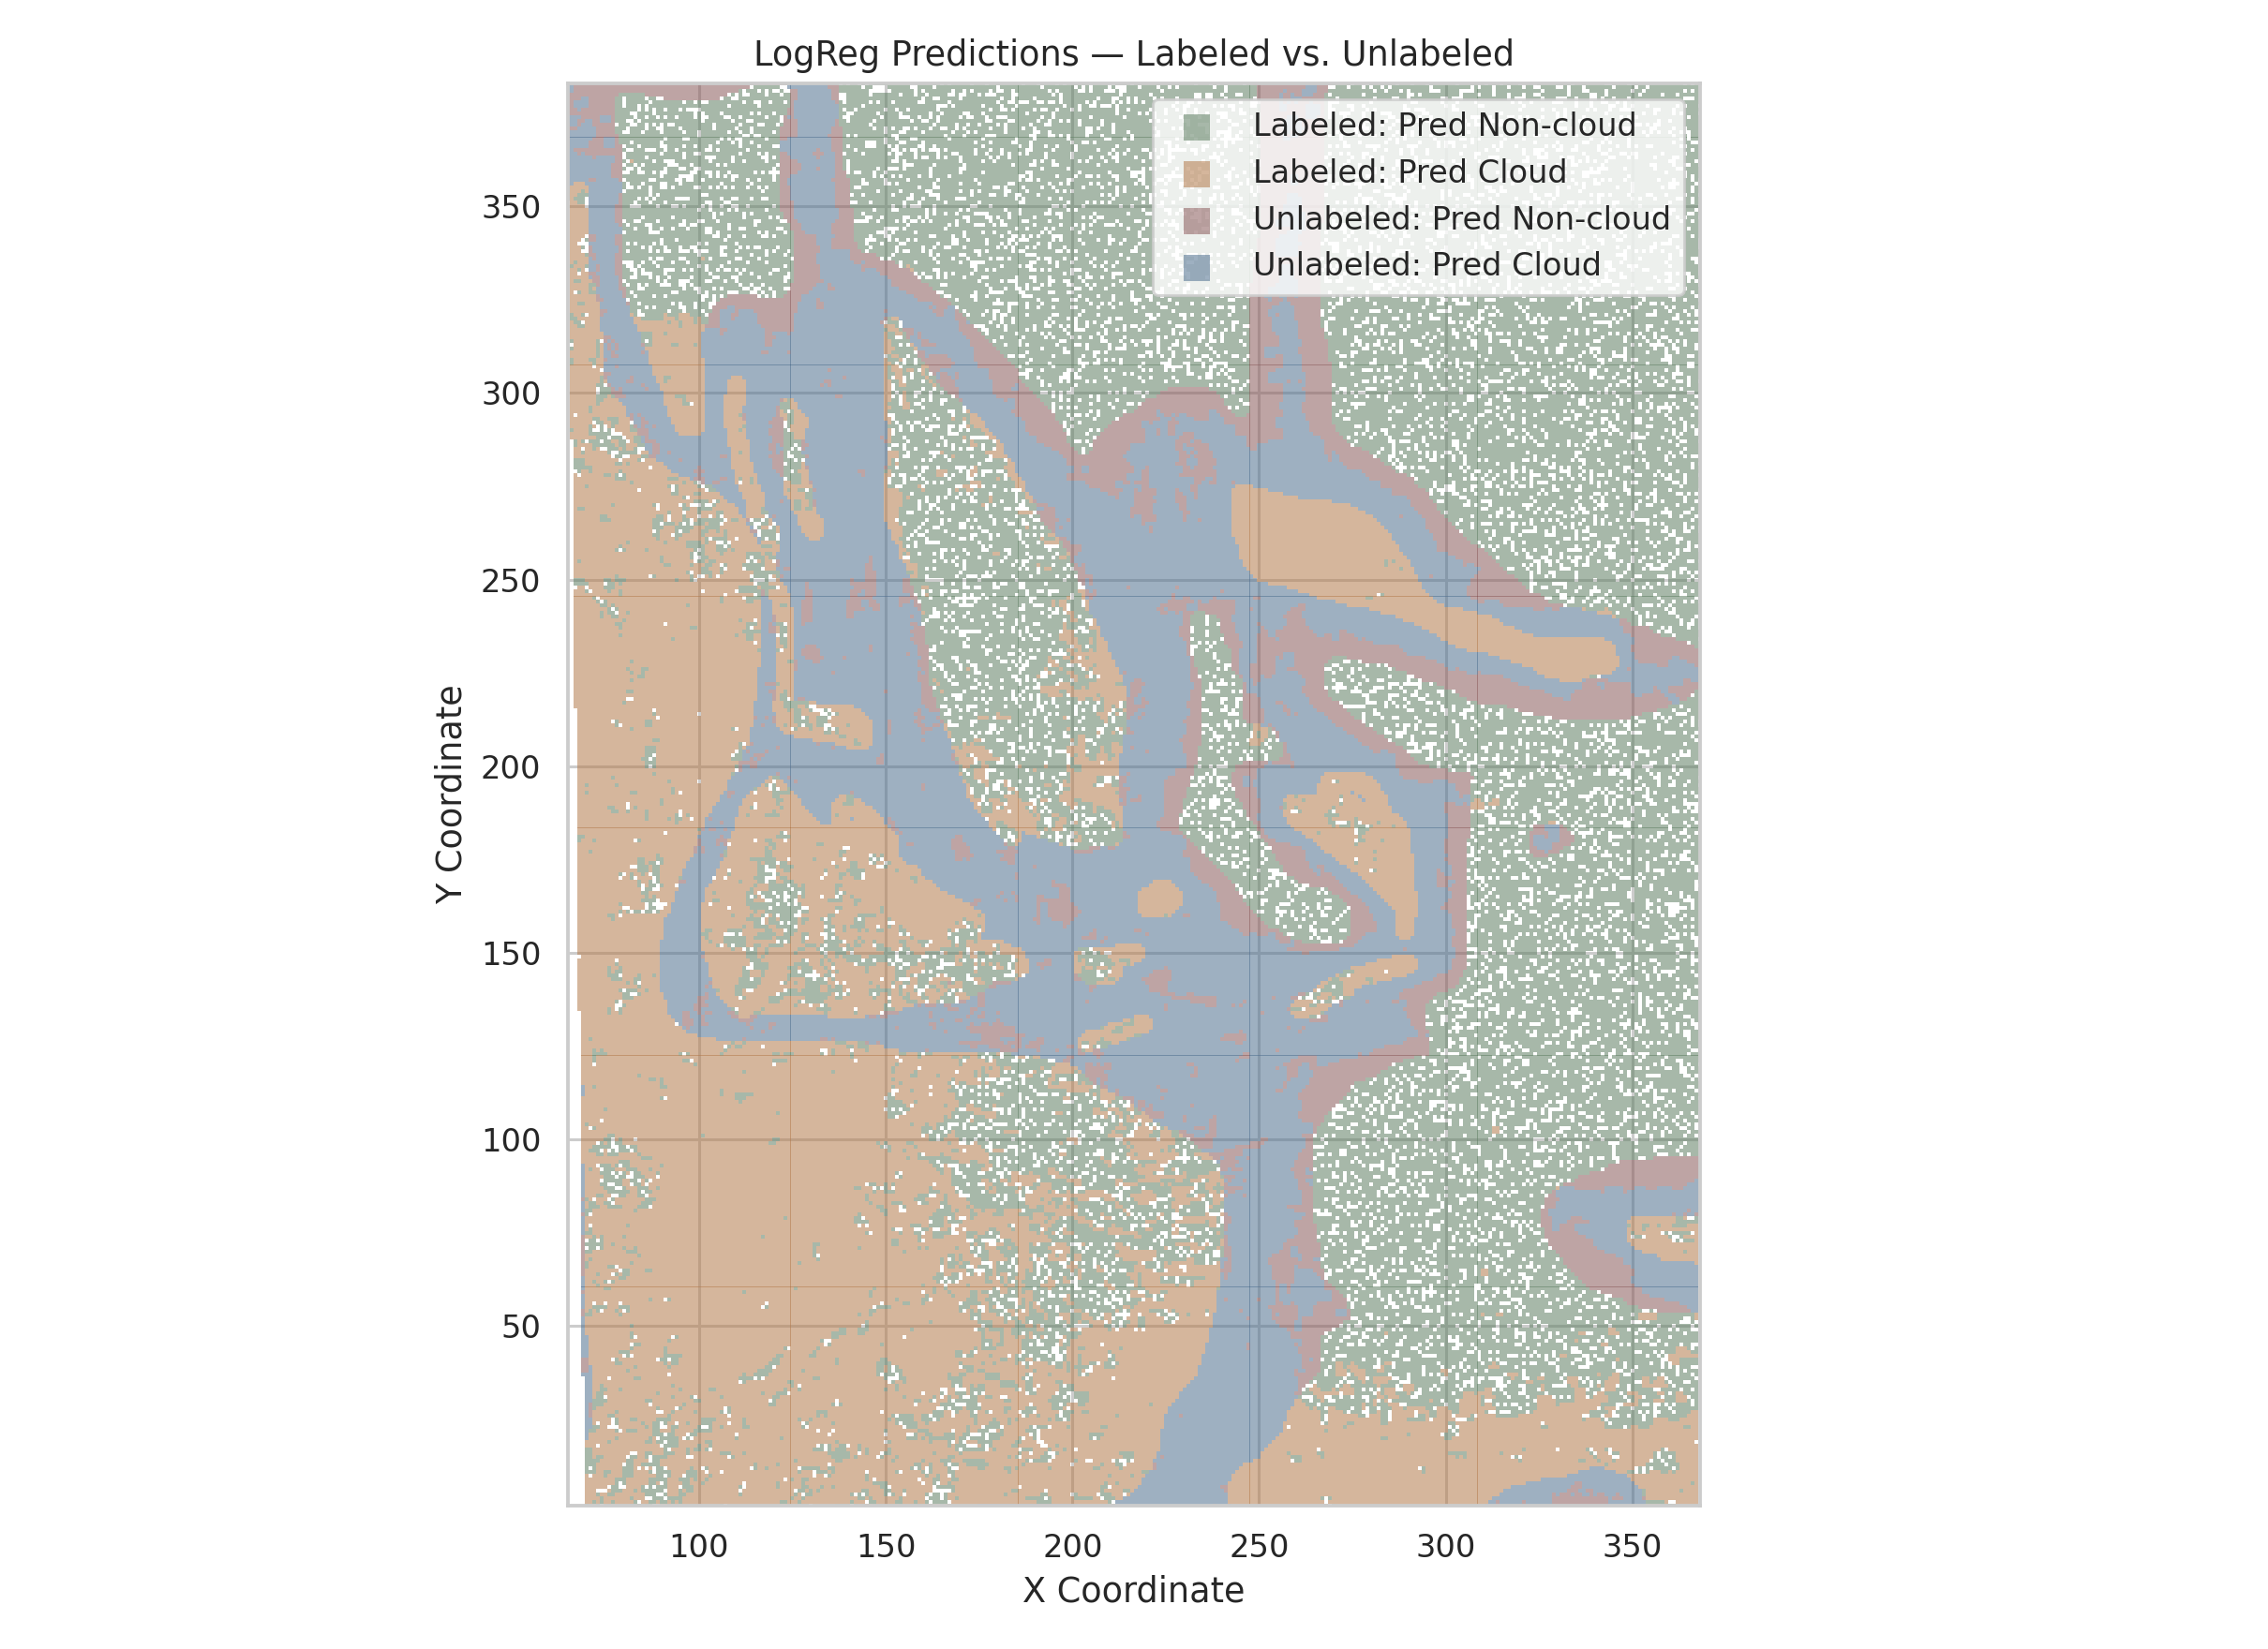
\includegraphics[width=\textwidth]{figures/model/logreg_labeled_vs_unlabeled.png}
\caption{Stepwise Logistic Regression spatial map}
\end{minipage}

\end{figure}


\begin{figure}[H]
    \centering
    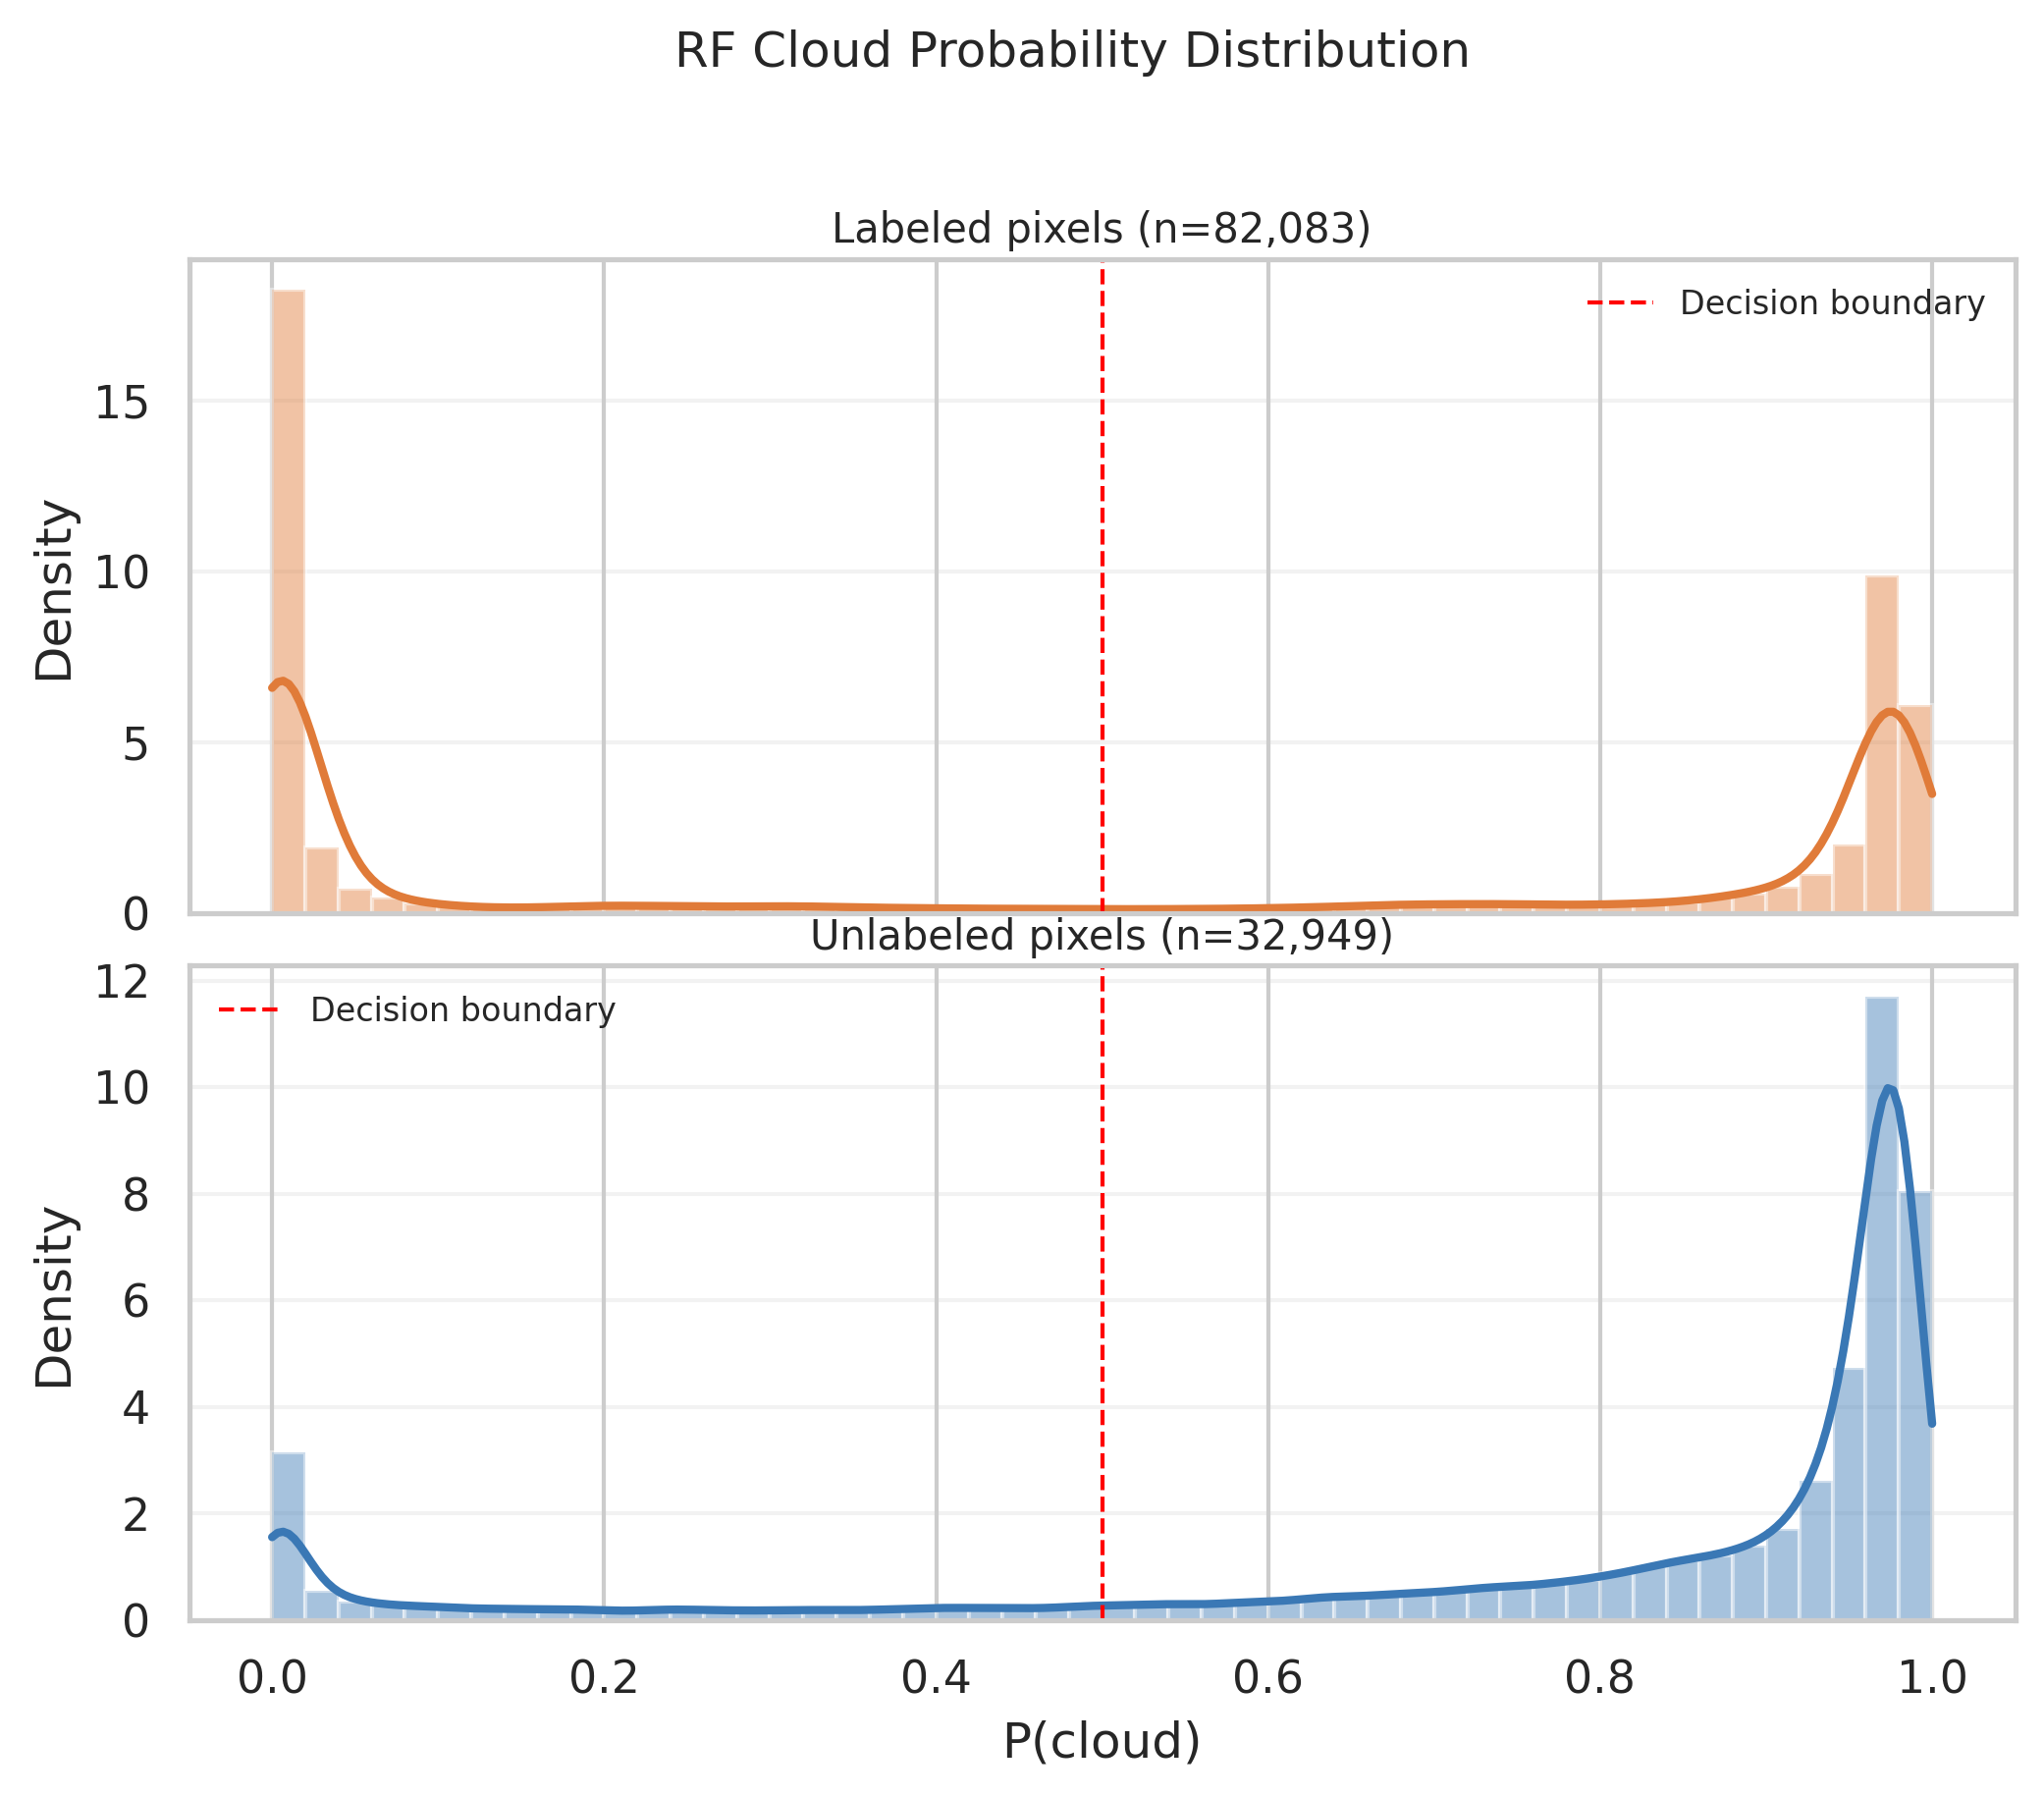
\includegraphics[width=0.62\textwidth]{figures/model/fig_model_rf_unlabeled_prob_hist.png}
    \caption{RF cloud probability distributions for labeled (top) and unlabeled (bottom) pixels in orbit \texttt{O013490}, shown in separate panels with a shared x-axis. Smooth curves are Gaussian KDE estimates ($h = 0.05\hat{\sigma}$, narrow bandwidth chosen to preserve the sharp bimodal peaks).}
    \label{fig:rf_unlabeled_hist}
\end{figure}

\begin{figure}[H]
    \centering
    \begin{minipage}{0.48\textwidth}
        \centering
        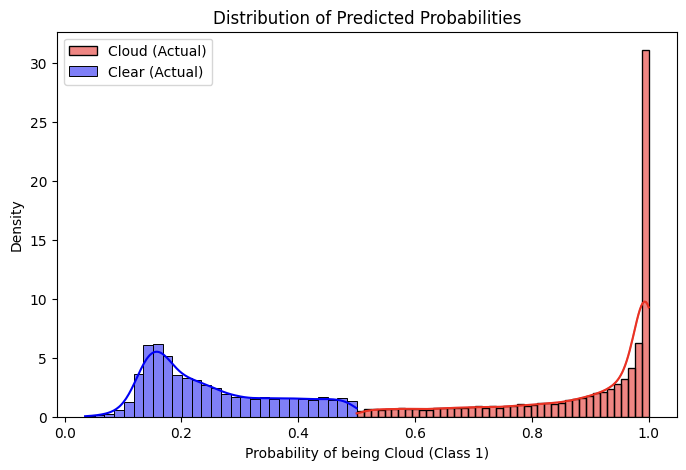
\includegraphics[width=\textwidth]{figures/model/hist_logreg.jpg}
        \caption{Logistic Regression cloud probability distributions for labeled and unlabeled pixels. Massing trends appear to be similar to RF results.}
        \label{fig:logreg_hist}
    \end{minipage} \hfill
    \begin{minipage}{0.48\textwidth}
        \centering
        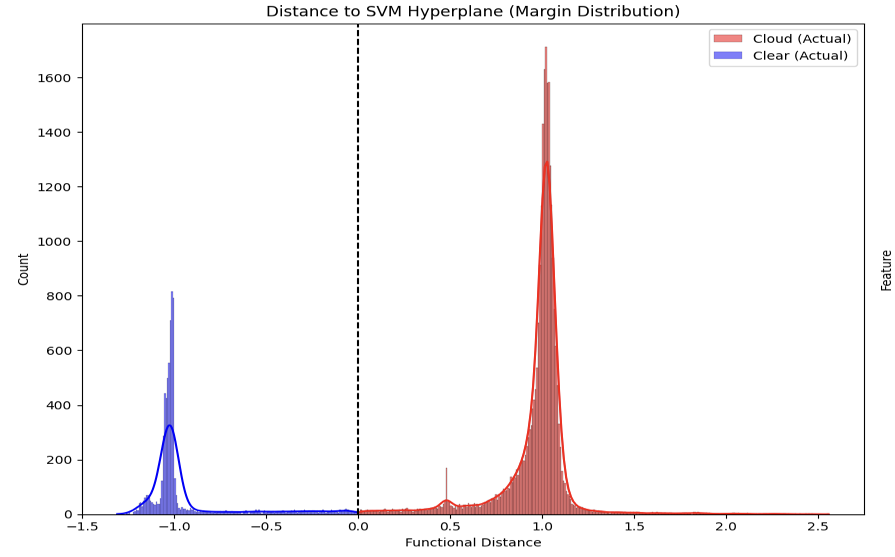
\includegraphics[width=\textwidth]{figures/model/svm_hyper.jpg}
        \caption{Distance from the unlabeled pixels to the dividing hyperplane in SVM model. Pattern of double peaks is also visible.}
        \label{fig:svm_hyper}
    \end{minipage}
\end{figure}

The strong cloud-skew (83\%) is consistent with where unlabeled pixels spatially appear: expert annotators tend to leave ambiguous labels at cloud boundaries and in partially-obscured regions, which are surrounded by labeled cloud pixels. The RF, drawing on spatial texture features (especially \texttt{SD}) and AE embeddings that encode local patch structure, reads these as cloud-like.


\subsubsection{Label Noise Robustness}
To assess sensitivity to annotation errors in the training set, we randomly flipped 5\% of training labels ($y \to -y$ with probability 0.05) and retrained the RF from scratch using the same hyperparameters. This was repeated 3 times with independent flip draws ($\approx$6,250 of 125,598 labels corrupted per run).

\begin{table}[H]
\centering
\begin{tabular}{lccc}
\toprule
\textbf{Condition} & \textbf{ROC AUC} & \textbf{F1} & \textbf{Accuracy} \\
\midrule
Clean labels        & 0.9941 & 0.9712 & 0.9720 \\
5\% flipped (mean)  & 0.9931 & 0.9725 & 0.9732 \\
5\% flipped (std)   & 0.0003 & 0.0009 & 0.0009 \\
\midrule
$\Delta$ (flipped $-$ clean) & $-$0.0010 & $+$0.0013 & $+$0.0012 \\
\bottomrule
\end{tabular}
\caption{RF test-set performance under 5\% training label flip, averaged over 3 independent repetitions. All metrics are evaluated on the clean temporal holdout (\texttt{O013490}).}
\label{tab:label_flip}
\end{table}

\begin{figure}[H]
    \centering
    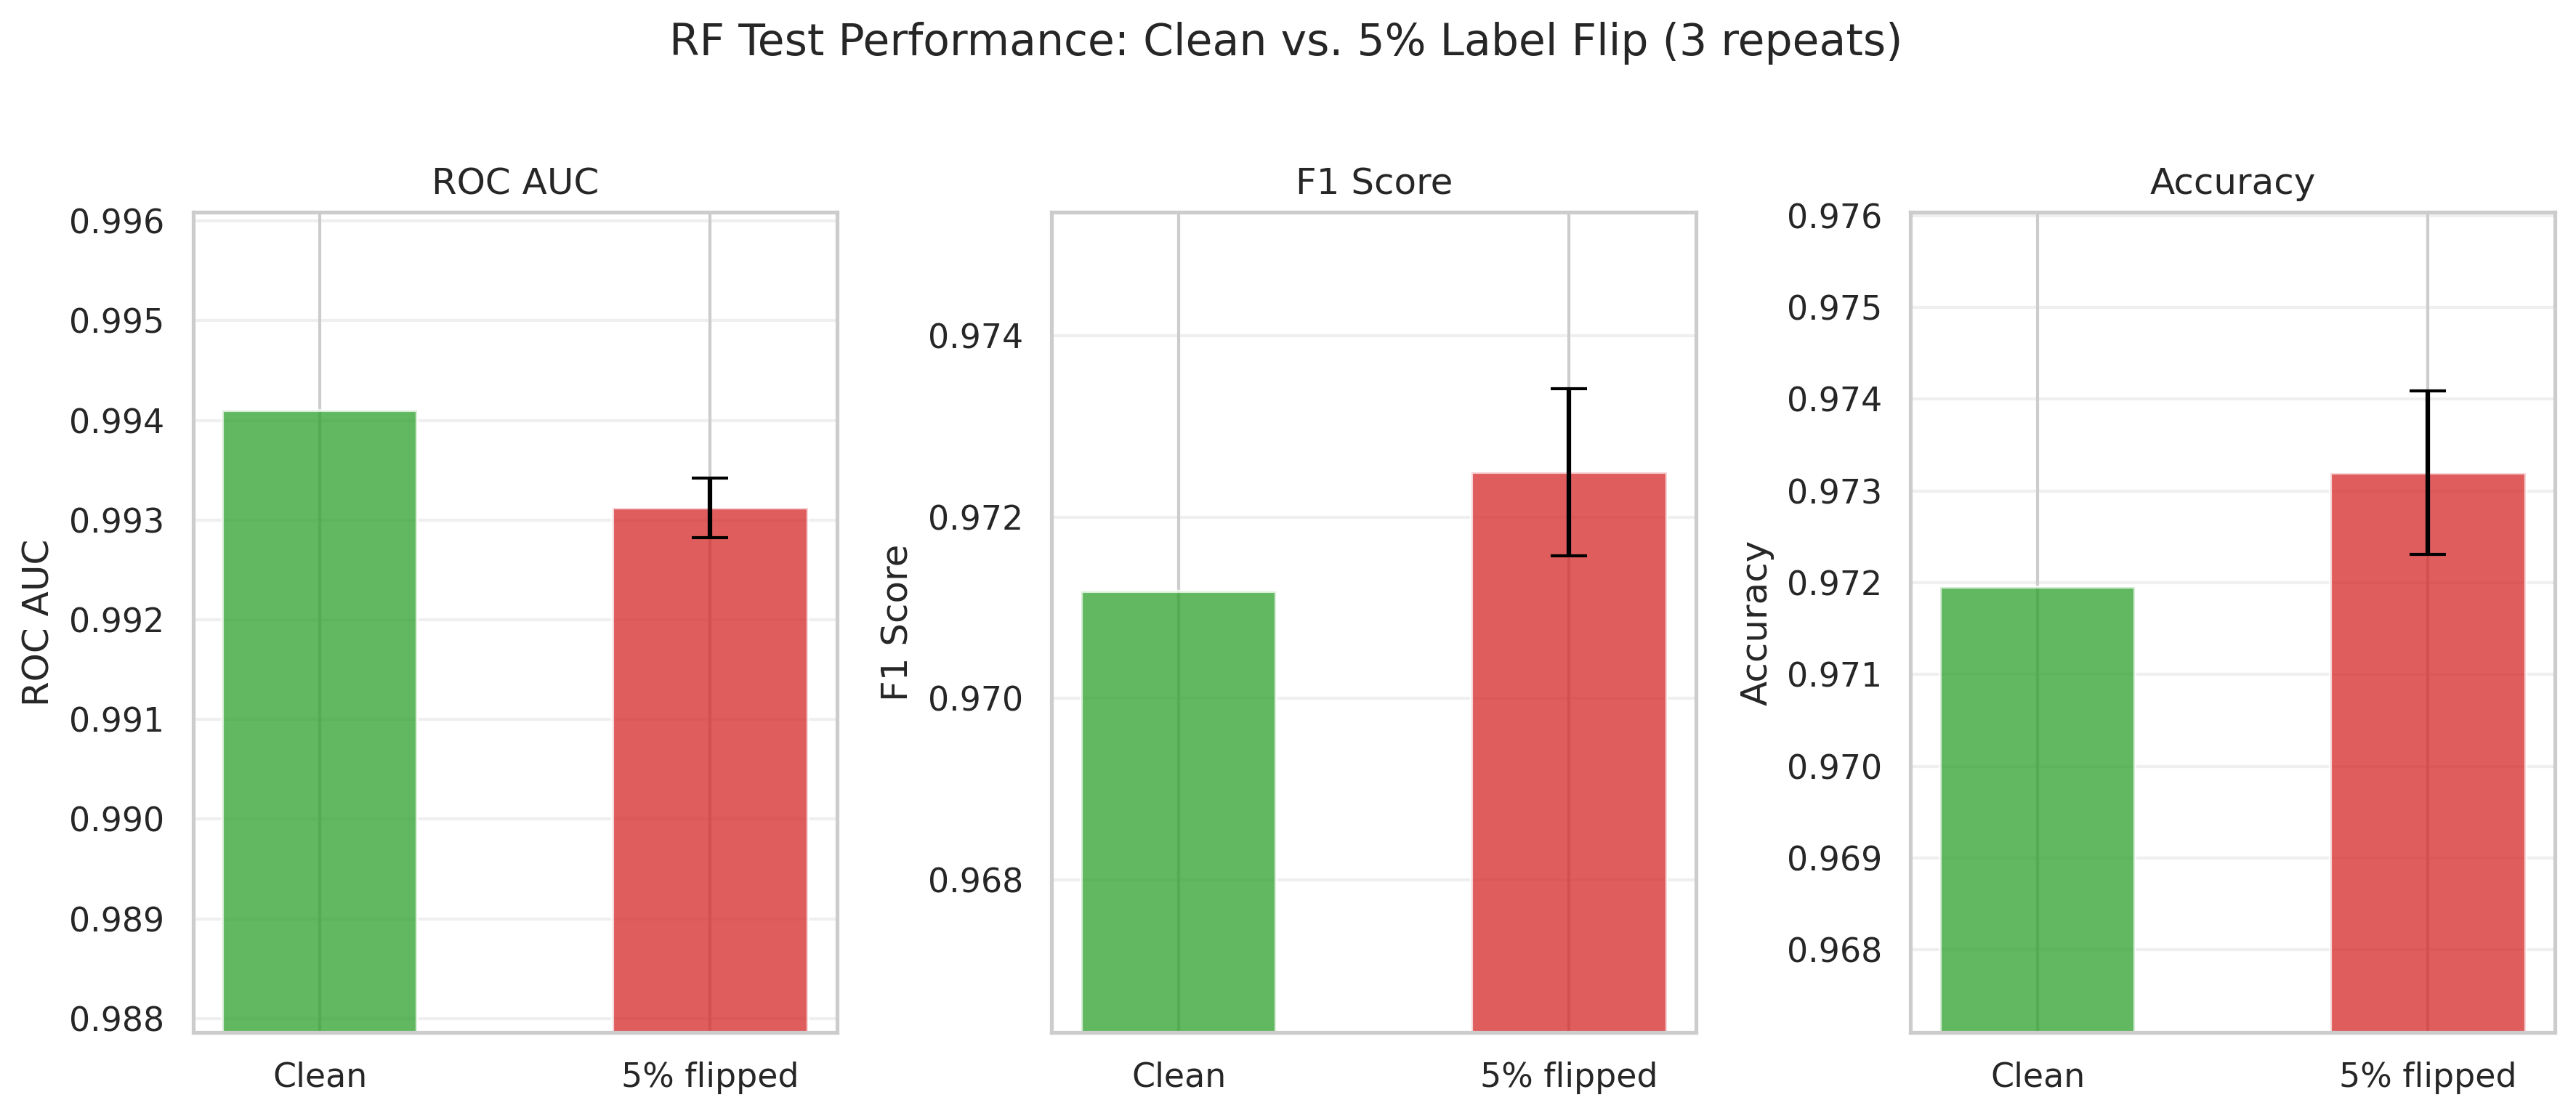
\includegraphics[width=0.9\textwidth]{figures/model/fig_model_rf_label_flip_stability.png}
    \caption{Bar chart comparing RF test metrics between clean and 5\%-flipped training labels. Error bars show standard deviation across 3 independent flip draws. The y-axis is zoomed to the relevant range to make the (small) differences visible.}
    \label{fig:label_flip}
\end{figure}


This robustness is expected from a Random Forest: the bagging mechanism means each tree is trained on a bootstrap sample, so the corrupted labels are spread across trees and their influence is diluted by the ensemble vote. In practice, this implies the model would remain reliable even if expert annotators disagreed on roughly 1 in 20 pixels. In other models other than ensemble learning, noise does compromises model performance to a certain extent. Logistic Regressions have all three metrics lowered after the flipping process. SVM exhibits a strong robustness against added noise. All three metrics have extremely little change compared to the original training result. 


% \begin{figure}[H]
%     \centering
%     \begin{minipage}{0.48\textwidth}
%         \centering
%         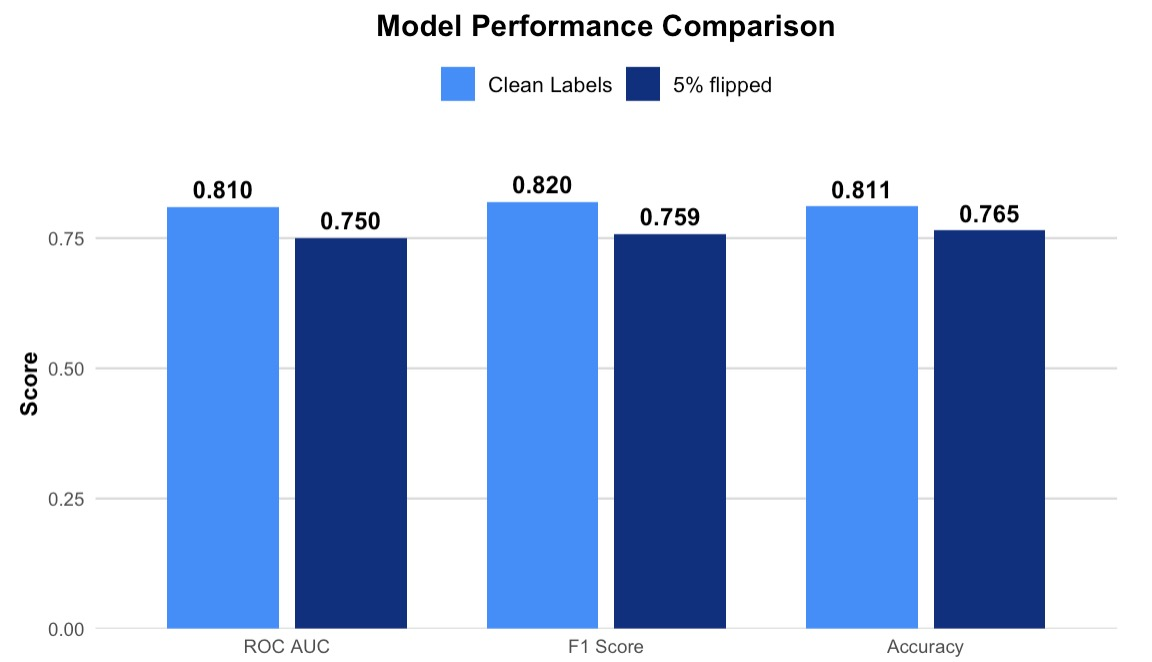
\includegraphics[width=\textwidth]{figures/model/logreg_comp.jpg}
%         \caption{Bar chart comparing Logistic Regression test metrics between clean and 5\%-flipped training labels.}
%         \label{fig:logreg_comp}
%     \end{minipage} \hfill
%     \begin{minipage}{0.48\textwidth}
%         \centering
%         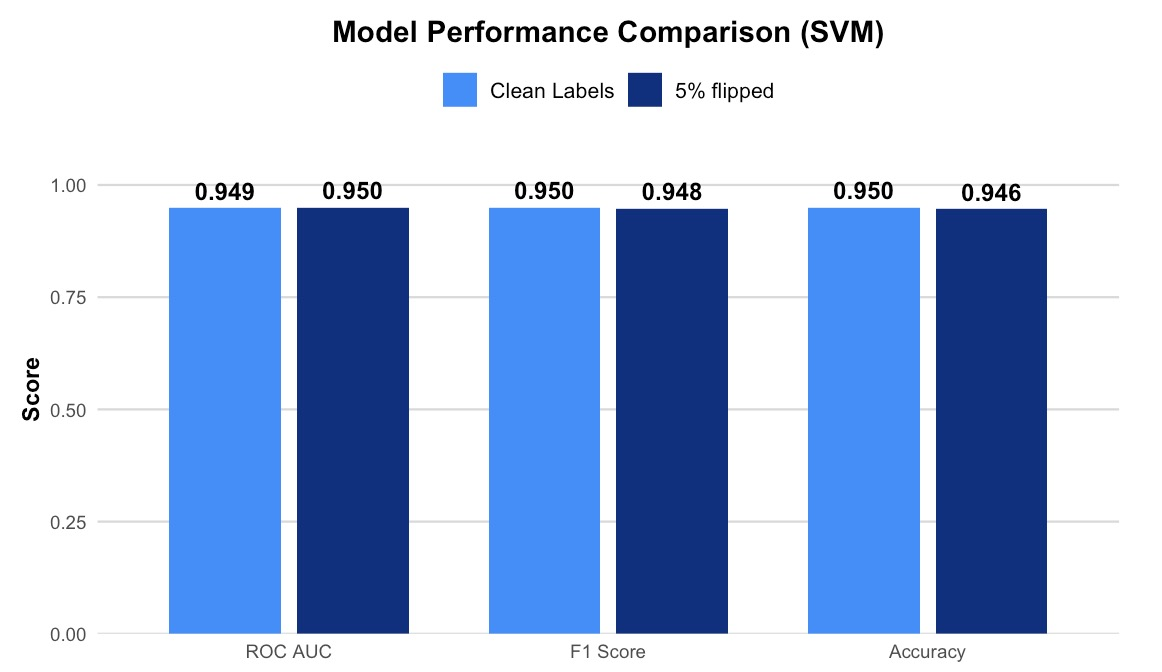
\includegraphics[width=\textwidth]{figures/model/svm_comp.jpg}
%         \caption{Bar chart comparing SVM test metrics between clean and 5\%-flipped training labels.}
%         \label{fig:svm_comp}
%     \end{minipage}
% \end{figure}



